\documentclass[dvipsnames, aspectratio=169]{beamer}
\usepackage[utf8]{inputenc}
\usepackage{listings}
\usepackage{comment}
\usepackage{soul}
%\usepackage{ulem}
\usepackage{subfig}
\usepackage{pgf-pie}
\setul{}{1pt}
\usepackage[oldenum, olditem]{paralist}
%allow even smaller text
\newcommand\tinytiny{\fontsize{4pt}{3}\selectfont}

\makeatletter
\let\old@lstKV@SwitchCases\lstKV@SwitchCases
\def\lstKV@SwitchCases#1#2#3{}
\makeatother
\usepackage{lstlinebgrd}
\makeatletter
\let\lstKV@SwitchCases\old@lstKV@SwitchCases

\lst@Key{numbers}{none}{%
    \def\lst@PlaceNumber{\lst@linebgrd}%
    \lstKV@SwitchCases{#1}%
    {none:\\%
     left:\def\lst@PlaceNumber{\llap{\normalfont
                \lst@numberstyle{\thelstnumber}\kern\lst@numbersep}\lst@linebgrd}\\%
     right:\def\lst@PlaceNumber{\rlap{\normalfont
                \kern\linewidth \kern\lst@numbersep
                \lst@numberstyle{\thelstnumber}}\lst@linebgrd}%
    }{\PackageError{Listings}{Numbers #1 unknown}\@ehc}}
\makeatother


%disclaimer for Sandia. uncomment and the whole blob goes away @ b80c116300122
\def\sandid{SAND2020-9031 PE}

% \title{Performance Portability with Kokkos}
\title{The Kokkos Lectures}

%BAD misuse of author field
\author{Module 7: Kokkos Tools}


\usetheme{kokkos}

\newif\ifshort
\newif\ifmedium
\newif\iffull
\newif\ifnotoverview

\newcommand{\TutorialDirectory}{\texttt{Intro-Full}}
\newcommand{\ExerciseDirectory}[1]{\texttt{Exercises/#1/}}
\newcommand{\TutorialClone}{\texttt{Kokkos/kokkos-tutorials/\TutorialDirectory}}

\definecolor{darkgreen}{rgb}{0.0, 0.5, 0.0}
\definecolor{darkred}{rgb}{0.8, 0.0, 0.0}
\definecolor{orange}{rgb}{0.8, 0.33, 0.0}
\definecolor{purple}{rgb}{0.60, 0.20, 0.80}
\colorlet{bodyColor}{blue!20}
\colorlet{patternColor}{orange!30}
\colorlet{policyColor}{green!30}

% http://tex.stackexchange.com/questions/144448/color-a-text-line-in-a-code-lstlisting
\lstnewenvironment{code}[1][]%
{
  %with txfonts: OT1/txr/m/n/10
  %with default fonts: OT1/cmr/m/n/10
  %\fontfamily{cmr}\selectfont
  %\showthe\font
   \noindent
   \minipage{\linewidth}
   %\vspace{0.5\baselineskip}
   \lstset{mathescape, escapeinside={<@}{@>},
moredelim=**[is][{\btHL[fill=patternColor]}]{@pattern}{@pattern},
moredelim=**[is][{\btHL[fill=red!30]}]{@warning}{@warning},
moredelim=**[is][{\btHL[fill=policyColor]}]{@policy}{@policy},
moredelim=**[is][{\btHL[fill=bodyColor]}]{@body}{@body},
moredelim=**[is][{\btHL[fill=red!30]}]{@warning}{@warning},
moredelim=**[is][\color{black}]{@black}{@black},
moredelim=**[is][\color{blue}]{@blue}{@blue},
moredelim=**[is][\bf]{@bold}{@bold},
moredelim=**[is][\it]{@italic}{@italic},
moredelim=**[is][\color{boldblue}\bf]{@boldblue}{@boldblue},
moredelim=**[is][\color{red}]{@red}{@red},
moredelim=**[is][\color{green}]{@green}{@green},
moredelim=**[is][\color{gray}]{@gray}{@gray},
moredelim=**[is][\color{darkgreen}]{@darkgreen}{@darkgreen},
moredelim=**[is][\color{darkred}]{@darkred}{@darkred},
moredelim=**[is][\color{orange}]{@orange}{@orange},
moredelim=**[is][\color{purple}]{@purple}{@purple},
keywords={},
#1}
}
{
  \endminipage
  %\vspace{1.0\baselineskip}
}

\makeatletter
\newif\ifATOlinebackground
\lst@Key{linebackground}{\tiny}{\def\ATOlinebackground{#1}\global\ATOlinebackgroundtrue}
\makeatother

\lstnewenvironment{shell}[1][]{%
  \global\ATOlinebackgroundfalse
  \lstset{language=sh,%
    showstringspaces=false,
    aboveskip=0pt,
    frame=none,
    numbers=none,
    belowskip=2pt,
    breaklines=true,
    #1,
    }
  %\ifATOlinebackground
  \lstset{linebackgroundcolor={
    \ATOlinebackground
  }}
  %\fi
  }{}

\lstnewenvironment{cmake}[1][]{%
  \global\ATOlinebackgroundfalse
  \lstset{language=sh,%
    showstringspaces=false,
    aboveskip=0pt,
    frame=none,
    numbers=none,
    belowskip=2pt,
    breaklines=true,
    #1,
    }
  %\ifATOlinebackground
  \lstset{linebackgroundcolor={
    \ATOlinebackground
  }}
  %\fi
  }{}

\newcommand{\inlinecode}[1]{{\lstset{basicstyle=\ttfamily,keywordstyle={},showstringspaces=false}\lstinline$#1$}}
\newcommand{\inlineshell}[1]{{\lstset{basicstyle=\ttfamily,keywordstyle={},showstringspaces=false}\lstinline$#1$}}

\setbeamercolor{block title}{fg=white, bg=SandiaLightBlue}
\setbeamercolor{block body}{bg=lightgray}
\setbeamercolor{block title alerted}{fg=white, bg=SandiaRed}
\setbeamercolor{block body alerted}{bg=lightgray}



%\usepackage[texcoord,grid,gridunit=mm,gridcolor=red!10,subgridcolor=green!10]{eso-pic}
\usepackage[absolute,overlay]{textpos}





% http://tex.stackexchange.com/questions/8851/how-can-i-highlight-some-lines-from-source-code

\usepackage{pgf, pgffor}
\usepackage{listings}
\usepackage{lstlinebgrd} % see http://www.ctan.org/pkg/lstaddons

\makeatletter
%%%%%%%%%%%%%%%%%%%%%%%%%%%%%%%%%%%%%%%%%%%%%%%%%%%%%%%%%%%%%%%%%%%%%%%%%%%%%%
%
% \btIfInRange{number}{range list}{TRUE}{FALSE}
%
% Test in int number <number> is element of a (comma separated) list of ranges
% (such as: {1,3-5,7,10-12,14}) and processes <TRUE> or <FALSE> respectively

\newcount\bt@rangea
\newcount\bt@rangeb

\newcommand\btIfInRange[2]{%
    \global\let\bt@inrange\@secondoftwo%
    \edef\bt@rangelist{#2}%
    \foreach \range in \bt@rangelist {%
        \afterassignment\bt@getrangeb%
        \bt@rangea=0\range\relax%
        \pgfmathtruncatemacro\result{ ( #1 >= \bt@rangea) && (#1 <= \bt@rangeb) }%
        \ifnum\result=1\relax%
            \breakforeach%
            \global\let\bt@inrange\@firstoftwo%
        \fi%
    }%
    \bt@inrange%
}
\newcommand\bt@getrangeb{%
    \@ifnextchar\relax%
        {\bt@rangeb=\bt@rangea}%
        {\@getrangeb}%
}
\def\@getrangeb-#1\relax{%
    \ifx\relax#1\relax%
        \bt@rangeb=100000%   \maxdimen is too large for pgfmath
    \else%
        \bt@rangeb=#1\relax%
    \fi%
}

%%%%%%%%%%%%%%%%%%%%%%%%%%%%%%%%%%%%%%%%%%%%%%%%%%%%%%%%%%%%%%%%%%%%%%%%%%%%%%
%
% \btLstHL<overlay spec>{range list}
%
% TODO BUG: \btLstHL commands can not yet be accumulated if more than one overlay spec match.
%
\newcommand<>{\btLstHL}[2]{%
  \only#3{\btIfInRange{\value{lstnumber}}{#1}{\color{#2}\def\lst@linebgrdcmd{\color@block}}{\def\lst@linebgrdcmd####1####2####3{}}}%
}%
\makeatother






% http://tex.stackexchange.com/questions/15237/highlight-text-in-code-listing-while-also-keeping-syntax-highlighting
%\usepackage[T1]{fontenc}
%\usepackage{listings,xcolor,beramono}
\usepackage{tikz}

\makeatletter
\newenvironment{btHighlight}[1][]
{\begingroup\tikzset{bt@Highlight@par/.style={#1}}\begin{lrbox}{\@tempboxa}}
{\end{lrbox}\bt@HL@box[bt@Highlight@par]{\@tempboxa}\endgroup}

\newcommand\btHL[1][]{%
  \begin{btHighlight}[#1]\bgroup\aftergroup\bt@HL@endenv%
}
\def\bt@HL@endenv{%
  \end{btHighlight}%
  \egroup
}
\newcommand{\bt@HL@box}[2][]{%
  \tikz[#1]{%
    \pgfpathrectangle{\pgfpoint{1pt}{0pt}}{\pgfpoint{\wd #2}{\ht #2}}%
    \pgfusepath{use as bounding box}%
    \node[anchor=base west, fill=orange!30,outer sep=0pt,inner xsep=1pt, inner ysep=0pt, rounded corners=3pt, minimum height=\ht\strutbox+1pt,#1]{\raisebox{1pt}{\strut}\strut\usebox{#2}};
  }%
}
\makeatother



\usetikzlibrary{calc}
\usepackage{xparse}%  For \NewDocumentCommand

% tikzmark command, for shading over items
\newcommand{\tikzmark}[1]{\tikz[overlay,remember picture] \node (#1) {};}

\makeatletter
\NewDocumentCommand{\DrawBox}{s O{}}{%
    \tikz[overlay,remember picture]{
    \IfBooleanTF{#1}{%
        \coordinate (RightPoint) at ($(left |- right)+(\linewidth-\labelsep-\labelwidth,0.0)$);
    }{%
        \coordinate (RightPoint) at (right.east);
    }%
    \draw[red,#2]
      ($(left)+(-0.2em,0.9em)$) rectangle
      ($(RightPoint)+(0.2em,-0.3em)$);}
}

\NewDocumentCommand{\DrawBoxWide}{s O{}}{%
    \tikz[overlay,remember picture]{
    \IfBooleanTF{#1}{%
        \coordinate (RightPoint) at ($(left |- right)+(\linewidth-\labelsep-\labelwidth,0.0)$);
    }{%
        \coordinate (RightPoint) at (right.east);
    }%
    \draw[red,#2]
      ($(left)+(-\labelwidth,0.9em)$) rectangle
      ($(RightPoint)+(0.2em,-0.3em)$);}
}

\NewDocumentCommand{\DrawBoxWideBlack}{s O{}}{%
    \tikz[overlay,remember picture]{
    \IfBooleanTF{#1}{%
        \coordinate (RightPoint) at ($(left |- right)+(\linewidth-\labelsep-\labelwidth,0.0)$);
    }{%
        \coordinate (RightPoint) at (right.east);
    }%
    \draw[black,#2]
      ($(left)+(-\labelwidth,0.9em)$) rectangle
      ($(RightPoint)+(0.2em,-0.3em)$);}
}
\makeatother

\usetikzlibrary{positioning}

\usetikzlibrary{shapes}

\hypersetup{
    colorlinks=true,
    linkcolor=blue,
    filecolor=magenta,
    urlcolor=cyan,
}



\shortfalse
\mediumtrue
\fulltrue
\notoverviewtrue

\begin{document}

\begin{frame}
	\titlepage
\end{frame}

\begin{frame}[fragile]{Welcome to Kokkos}

\textbf{Online Resources}:

\begin{itemize}
        \item \url{https://github.com/kokkos}:
                \begin{itemize}
                        \item Primary Kokkos GitHub Organization
                \end{itemize}
        \item \url{https://github.com/kokkos/kokkos-tutorials/wiki/Kokkos-Lecture-Series}:
                \begin{itemize}
			\item{Slides, recording and Q\&A for the Lectures}
                \end{itemize}
        \item \url{https://kokkos.github.io/kokkos-core-wiki}:
                \begin{itemize}
                        \item Wiki including API reference
                \end{itemize}
        \item \url{https://github.com/kokkos/kokkos-tools/wiki}:
                \begin{itemize}
                        \item Kokkos Tools Wiki
                \end{itemize}
        \item \url{https://kokkosteam.slack.com}:
                \begin{itemize}
                        \item Slack channel for Kokkos.
                        \item Please join: fastest way to get your questions answered.
                        \item Can whitelist domains, or invite individual people.
                \end{itemize}
\end{itemize}

\end{frame}


\begin{frame}[fragile]{Lecture Series Outline}

\begin{itemize}
        \item Module 1: Introduction, Building and Parallel Dispatch
        \item Module 2: Views and Spaces
        \item Module 3: Data Structures + MultiDimensional Loops
        \item Module 4: Hierarchical Parallelism
        \item Module 5: Tasking, Streams and SIMD
        \item Module 6: Internode: MPI and PGAS
        \item \textbf{Module 7: Tools: Profiling, Tuning and Debugging}
        \item Module 8: Kernels: Sparse and Dense Linear Algebra
        \item Module 9: Fortran inter-op
\end{itemize}

\end{frame}

\begin{frame}{Module 6 Summary}
\textbf{Simple MPI and Kokkos Interaction is easy!}
\begin{itemize}
  \item Simply pass \texttt{data()} of a View to MPI functions plus its size.
  \begin{itemize}
    \item But it better be a contiguous View!
  \end{itemize}
  \item Initialize Kokkos after MPI, and finalize it before MPI
\end{itemize}

\vspace{10pt}
\textbf{Overlapping communication and computation possible}
\begin{itemize}
  \item Use Execution Space instances to overlap packing/unpacking with other computation.
  \item Order operations to maximize overlapping potential. 
\end{itemize}
\end{frame}

\begin{frame}[fragile]{Module 6 Summary}
\textbf{Fortran Language Compatibility Layer}
\begin{itemize}
  \item Initialize Kokkos from Fortran via \texttt{kokkos\_initialize} and \texttt{kokkos\_finalize}
  \item \texttt{nd\_array\_t} is a representation of a \texttt{Kokkos::View}
  \item Create \texttt{nd\_array\_t} from a Fortran array via \texttt{to\_nd\_array}
  \item Allocate \texttt{Kokkos::DualView} in Fortran with \texttt{kokkos\_allocate\_dualview}
\end{itemize}


  \vspace{10pt}
  \textbf{The Python Interop}
  \begin{itemize}
    \item Initialize and Finalize Kokkos from Python
    \item Create Views from Python
    \item Alias Kokkos Views with NumPy arrays
    \item \textbf{This is in pre-release: ask us for access.}
  \end{itemize}
\end{frame}

\begin{frame}{Module 7: Learning objectives}
  \begin{block}{Simple Tools Usage}
    \begin{itemize}
    \item How to dynamically load a Kokkos Tool.
    \item Simple Profiling and Debugging.
    \item Leveraging the KokkosP instrumentation for third party tools.
  \end{itemize}
  \end{block}

  \begin{block}{Kokkos Tuning}
  \begin{itemize}
    \item Learn to auto-tune runtime parameters.
  \end{itemize}
  \end{block}

  \begin{block}{Build Your Own Tool}
  \begin{itemize}
    \item Learn how to build your own tools.
  \end{itemize}
  \end{block}

  \begin{block}{Leveraging Static Analysis}
  \begin{itemize}
    \item How to use Kokkos' LLVM tools for static analysis.
  \end{itemize}
  \end{block}
\end{frame}

\begin{frame}[fragile]

  {\Huge Kokkos Tools}

  \vspace{10pt}

  {\large Leveraging Kokkos' built-in instrumentation.}

  \vspace{20pt}

  \textbf{Learning objectives:}
  \begin{itemize}
    \item {The need for Kokkos-aware tools.}
    \item {How instrumentation helps.}
    \item {Simple profiling tools.}
    \item {Simple debugging tools.}
  \end{itemize}

  \vspace{-20pt}

\end{frame}

%==========================================================================

\begin{frame}[fragile]{Profiling C++ Code}
  \textbf{Output from NVIDIA NVProf for Trilinos Tpetra}

  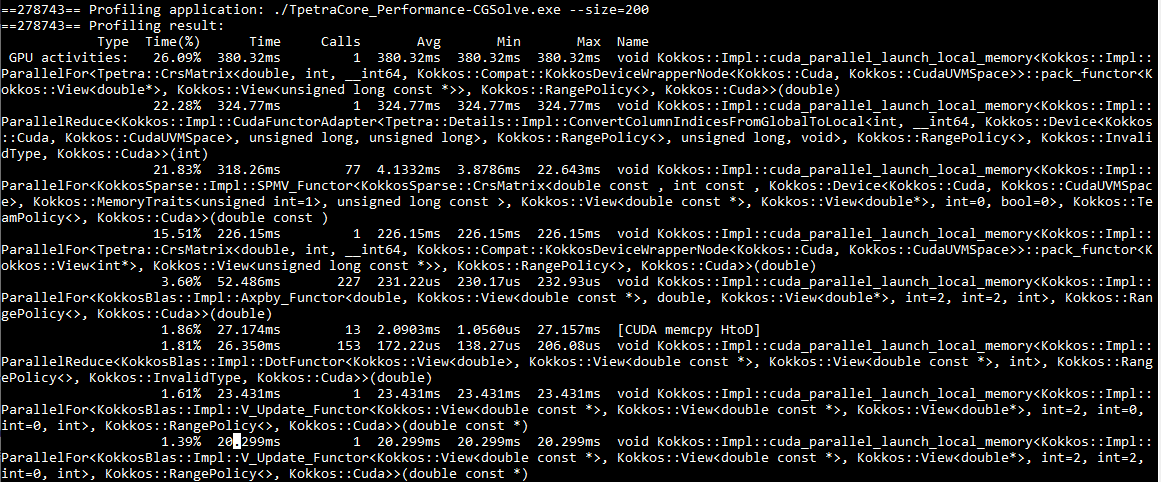
\includegraphics[width=\textwidth]{../figures/tools-tpetra-nvprof}

\vspace{5pt}
\pause
\textit{What are those Kernels doing?}
\end{frame}

%==========================================================================

\begin{frame}[fragile]{Why is it so bad?}
  \textbf{Generic code obscures what is happening from the tools}

  Historically a lot of profiling tools are coming from a Fortran and C world:

  \begin{itemize}
    \item Focused on functions and variables
    \item C++ has a lot of other concepts:
    \begin{itemize}
      \item Classes with member functions
      \item Inheritance
      \item Template Metaprogramming
    \end{itemize}
    \item Abstraction Models (Generic Programming) obscure things
    \begin{itemize}
      \item From a profiler perspective interesting stuff happens in the abstraction layer (e.g. \texttt{\#pragma omp parallel})
      \item Symbol names get really complex due to deep template layers  
    \end{itemize}
  \end{itemize}

\end{frame}

%==========================================================================

\begin{frame}[fragile]{Instrumentation to the Rescue}
  \textbf{Instrumentation enables context information to reach tools.}

  \vspace{5pt}
  Most profiling tools have an instrumentation interface

  \begin{itemize}
    \item E.g. nvtx for NVIDIA, ITT for Intel.
    \item Allows to name regions
    \item Sometimes can mark up memory operations.
  \end{itemize}

  \pause
  \vspace{5pt}
  \begin{block}{KokkosP}
    Kokkos has its own instrumentation interface KokkosP, which can be used to write tools.
  \end{block}

  \begin{itemize}
    \item Knows about parallel dispatch
    \item Knows about allocations, deallocations and deep\_copy
    \item Provides region markers
    \item Leverages naming information (kernels, Views)
  \end{itemize}

\end{frame}

%==========================================================================

\begin{frame}[fragile]{The Kokkos Tools}
  There are two components to Kokkos Tools: the KokkosP instrumentation interface and the actual Tools. 

  \vspace{10pt}
  \textbf{KokkosP Interface}

  \begin{itemize}
    \item The internal instrumentation layer of Kokkos.
    \item Always available even in release builds.
    \item Zero overhead if no tool is loaded.
  \end{itemize}

  \vspace{5pt}
  \textbf{Kokkos Tools}
  \begin{itemize}
    \item Tools leveraging the KokkosP instrumentation layer.
    \item Are loaded at runtime by Kokkos.
    \begin{itemize}
      \item Set \texttt{KOKKOS\_TOOLS\_LIBS} environment variable to load a shared library.
      \item Compile tools into the executable and use the API callback setting mechanism. 
    \end{itemize}
  \end{itemize}
\end{frame}

%==========================================================================

\begin{frame}[fragile]{How does it Work}
Download tools from \url{https://github.com/kokkos/kokkos-tools}

\begin{itemize}
  \item Tools are largely independent of the Kokkos configuration
    \begin{itemize}
      \item May need to use the same C++ standard library.
      \item Use the same tool for CUDA and OpenMP code for example.
     \end{itemize}
  \item We recommend you build the tools with CMake
\begin{lstlisting}
cd kokkos-tools && cmake -B build
cmake --build build --parallel 4
cmake --install build --prefix /where/to/install/the/tools
\end{lstlisting}
\end{itemize}

\vspace{5pt}
Loading Tools:
\begin{itemize}
  \item Set \texttt{KOKKOS\_TOOLS\_LIBS} environment variable to the full path to the shared library of the tool.
  \item Kokkos dynamically loads symbols from the library during \texttt{initialize} and fills function pointers.
  \item If no tool is loaded the overhead is a function pointer comparison to \texttt{nullptr}.
\end{itemize}

\end{frame}



%==========================================================================

\begin{frame}[fragile]{An Example Code}
\begin{code}[keywords={popRegion,pushRegion,Profiling,parallel_for,deep_copy,parallel_scan,parallel_reduce,K_1,K_2,Init_A,tmp,a,h_a}]
View<double*> a("A",N);
View<double*, HostSpace> h_a = create_mirror_view(a);

Profiling::pushRegion("Setup");
parallel_for("Init_A",RangePolicy<h_exec_t>(0,N),
  KOKKOS_LAMBDA(int i) { h_a(i) = i; });
deep_copy(a,h_a);
Profiling::popRegion();

Profiling::pushRegion("Iterate");
for(int r=0; r<10; r++) {
  View<double*> tmp("Tmp",N);
  parallel_scan("K_1",RangePolicy<exec_t>(0,N),
    KOKKOS_LAMBDA(int i, double& lsum, bool f) {
      if(f) tmp(i) = lsum;
      lsum += a(i);
  });
  double sum;
  parallel_reduce("K_2",N, KOKKOS_LAMBDA(int i, double& lsum) {
    lsum += tmp(i);
  },sum);
}
Profiling::popRegion();
\end{code}
\end{frame}

%==========================================================================

\begin{frame}[fragile]{An Example Code: Nvprof}
  Output of: \texttt{nvprof ./test.cuda}

  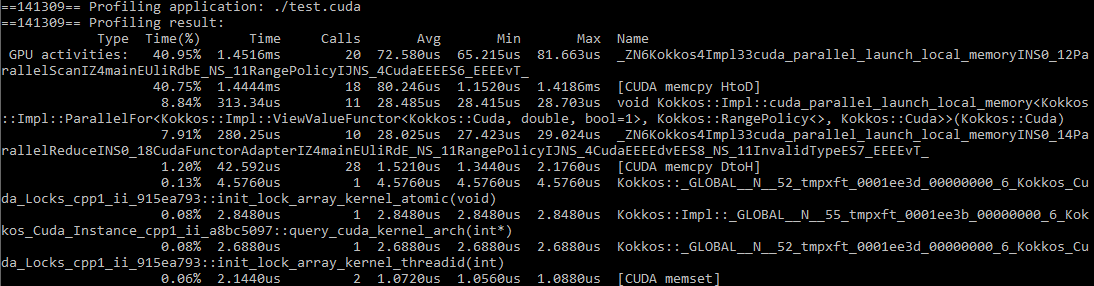
\includegraphics[width=\textwidth]{../figures/tools-nvprof-simple-code}

  \pause
Let us make one larger:

\vspace{-4pt}
\begin{code}
_ZN6Kokkos4Impl33cuda_parallel_launch_local_memoryINS0
_14ParallelReduceINS0_18CudaFunctorAdapterIZ4mainEUliRdE
_NS_11RangePolicyIJNS_4CudaEEEEdvEES8_NS_11InvalidTypeES7_EEEEvT_
\end{code}

And demangled:

\vspace{-4pt}
\begin{code}
void Kokkos::Impl::cuda_parallel_launch_local_memory
<Kokkos::Impl::ParallelReduce<Kokkos::Impl::CudaFunctorAdapter
<main::{lambda(int, double&)#1}, Kokkos::RangePolicy<Kokkos::Cuda>, 
double, void>, Kokkos::Cuda, Kokkos::InvalidType, Kokkos::RangePolicy> >
(Kokkos::Impl::ParallelReduce<Kokkos::Impl::CudaFunctorAdapter<
main::{lambda(int, double&)#1}, Kokkos::RangePolicy<Kokkos::Cuda>, 
double, void>, Kokkos::Cuda, Kokkos::InvalidType, Kokkos::RangePolicy>)
\end{code}
\end{frame}

%==========================================================================

\begin{frame}[fragile]{An Example Code}
\textbf{Aaa this is horrifying can't we do better??}

\pause
\vspace{10pt}
\textbf{Lets use SimpleKernelTimer from Kokkos Tools:}

\begin{itemize}
\item Simple tool producing a summary similar to nvprof
\item Good way to get a rough overview of whats going on
\item Writes a file \texttt{HOSTNAME-PROCESSID.dat} per process
\item Use the reader accompanying the tool to read the data
\end{itemize}

Usage:

\begin{code}[mathescape=false]
  git clone git@github.com:kokkos/kokkos-tools
  cd kokkos-tools/profiling/simple_kernel_timer
  make
  export KOKKOS_TOOLS_LIBS=${PWD}/kp_kernel_timer.so
  export PATH=${PATH}:${PWD}
  cd ${WORKDIR}
  ./text.cuda
  kp_reader *.dat
\end{code}

\end{frame}

%==========================================================================

\begin{frame}[fragile]{An Example Code}

Output from SimpleKernelTimer:
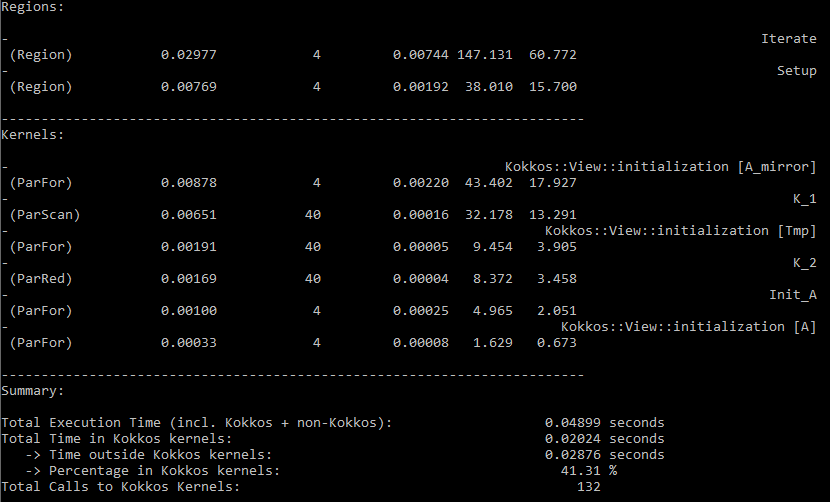
\includegraphics[width=0.85\textwidth]{../figures/tools-kerneltimer-simple-code}

\pause
\vspace{5pt}
Will introduce \textit{Regions} later.

\begin{block}{Kernel Naming}
Naming Kernels avoid seeing confusing Profiler output!
\end{block}

%\begin{code}[keywords={popRegion,pushRegion,Profiling,parallel_for,deep_copy,parallel_scan,parallel_reduce,K_1,K_2,Init_A,tmp,a,h_a}]
%Regions:
%- Iterate (REGION)   0.007105 1 0.007105 202.569506 67.768858
%- Setup (REGION)   0.001906 1 0.001906 54.340290 18.179337
%
%-------------------------------------------------------------------------
%Kernels:
%- K_1 (ParScan)  0.001583 10 0.000158 45.136293 15.100175
%- Kokkos::View::initialization [A_mirror] (ParFor)   0.000809 1 0.000809 23.064374 7.716099
%- Kokkos::View::initialization [Tmp] (ParFor)   0.000419 10 0.000042 11.943444 3.995634
%- K_2 (ParRed)   0.000386 10 0.000039 11.018965 3.686353
%- Init_A (ParFor)   0.000238 1 0.000238 6.784039 2.269575
%- Kokkos::View::initialization [A] (ParFor)   0.000072 1 0.000072 2.052886 0.686785
%
%-------------------------------------------------------------------------
%Summary:
%Total Execution Time (incl. Kokkos + non-Kokkos): 0.01048 s
%Total Time in Kokkos kernels:                     0.00351 s
%   -> Time outside Kokkos kernels:                0.00698 s
%   -> Percentage in Kokkos kernels:               33.45 %
%Total Calls to Kokkos Kernels:                    33
%\end{code}
\end{frame}

%==========================================================================

\begin{frame}[fragile]{Revisiting Tpetra}

Lets look at Tpetra again with the Simple Kernel Timer Loaded:

\vspace{10pt}
At the top we get Region output:

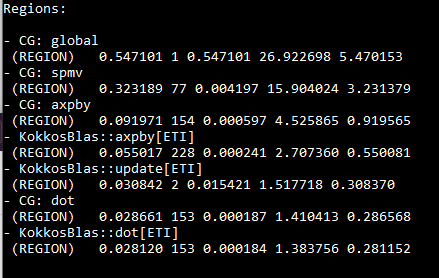
\includegraphics[width=0.7\textwidth]{../figures/tools-tpetra-regions}
\end{frame}

%==========================================================================

\begin{frame}[fragile]{Revisiting Tpetra}


Then we get kernel output:
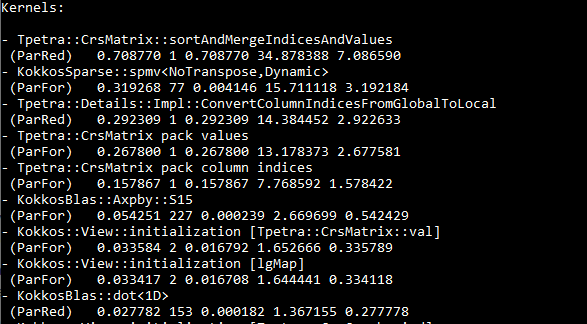
\includegraphics[width=\textwidth]{../figures/tools-tpetra-kernels}
\end{frame}

%==========================================================================

\begin{frame}[fragile]{Memory Utilization}
\textbf{Understanding MemorySpace Utilization is critical}

\vspace{10pt}
Three simple tools for understanding memory utilization:
\begin{itemize}
  \item MemoryHighWaterMark: just the maximum utilization for each memory space.
  \item MemoryUsage: Timeline of memory usage.
  \item MemoryEvents: allocation, deallocation and deep\_copy.
  \begin{itemize}
    \item Name, Memory Space, Pointer, Size
  \end{itemize}
\end{itemize}

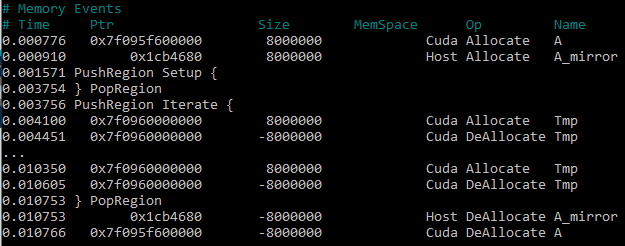
\includegraphics[width=0.8\textwidth]{../figures/tools-memevents-simple-code}
\end{frame}

%==========================================================================

\begin{frame}[fragile]{Push/Pop Regions}
	\textbf{Adding region markers to capture more code structure}

Region Markers are helpful to:
\begin{itemize}
  \item Find where time is spent outside of kernels.
  \item Group Kernels which belong together.
  \item Structure code profiles.
  \begin{itemize}
     \item For example bracket \textit{setup} or \textit{solve} phase. 
  \end{itemize}
\end{itemize}

\pause
\vspace{10pt}
Simple Push/Pop interface:
\begin{code}
  Kokkos::Profiling::pushRegion("Label");
  ...
  Kokkos::Profiling::popRegion();
\end{code}
\end{frame}

%==========================================================================

\begin{frame}[fragile]{Space Time Stack}
The simplest tool to leverage regions is the \textbf{Space Time Stack}:

\begin{itemize}
  \item \textbf{Bottom Up} and \textbf{Top Down} data representation
  \item Can do MPI aggregation if compiled with MPI support
  \item Also aggregates memory utilization info.
\end{itemize}

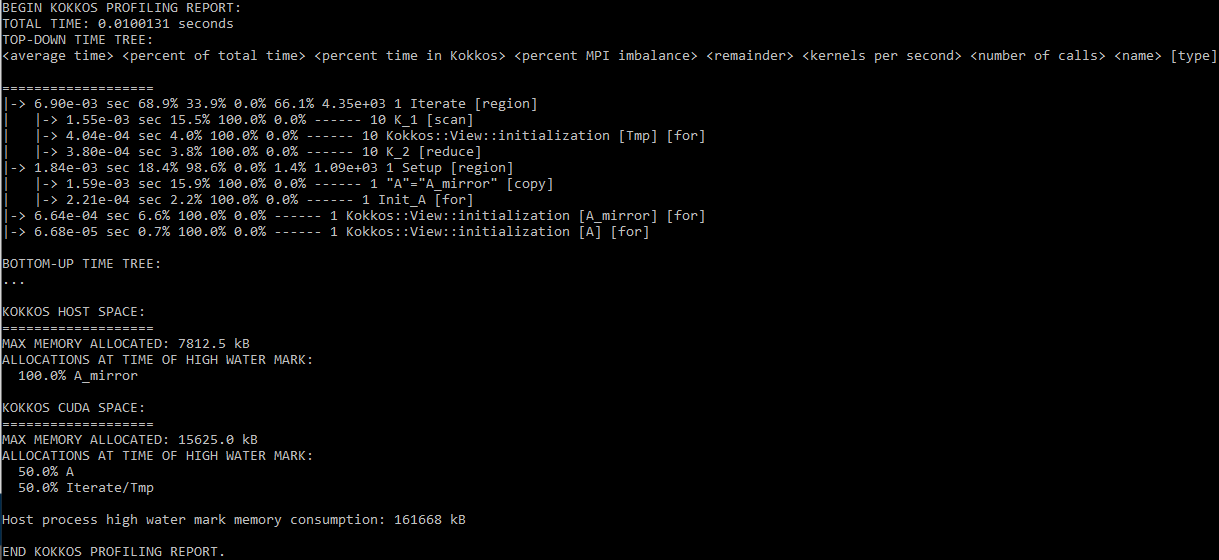
\includegraphics[width=\textwidth]{../figures/tools-sts-bup2-simple-code}

\end{frame}

%==========================================================================

\begin{frame}[fragile]{The Delayed Error Problem}
\textbf{Non-Blocking Dispatch implies asynchronous error reporting!}

\begin{code}[keywords={parallel_for,parallel_reduce,pushRegion,popRegion,Profiling,int,for},linebackgroundcolor={\btLstHL{3-4}{darkred!20}}]
Profiling::pushRegion("Iterate");
for(int r=0; r<10; r++) {
  parallel_for("K_1",2*N, KOKKOS_LAMBDA(int i) {a(i) = i;});  
  printf("Passed point A\n");
  double sum;
  parallel_reduce("K_2",N, KOKKOS_LAMBDA(int i, double& lsum) {
    lsum += a(i); },sum);
}
Profiling::popRegion();
\end{code}

Output of the run:
\begin{code}[linebackgroundcolor={\btLstHL{2}{darkred!20}}]
./test.cuda
Passed point A
terminate called after throwing an instance of 'std::runtime_error'
  what():  cudaStreamSynchronize(m_stream) error( cudaErrorIllegalAddress): 
  an illegal memory access was encountered 
    Kokkos/kokkos/core/src/Cuda/Kokkos_Cuda_Instance.cpp:312
Traceback functionality not available
Aborted (core dumped)
\end{code}
\end{frame}

%==========================================================================

\begin{frame}[fragile]{Kernel Logger for Debugging}
\begin{block}{Debugging with Tools}
Kokkos Tools can be used to implement Debugging functionality.
\end{block}

\pause
The KernelLogger is a tool to localize errors and check the actual runtime flow of a code.
\begin{itemize}
  \item As other tools it inserts fences - which check for errors.
  \item Prints out Kokkos operations as they happen.
\end{itemize}

\pause
Output from the above test case with KernelLogger:

\vspace{-5pt}
\begin{code}
KokkosP: Allocate<Cuda> name: A pointer: 0x7f598b800000 size: 8000000
KokkosP: Executing parallel-for kernel on device 0 with unique execution identifier 0
KokkosP: Kokkos::View::initialization [A]
KokkosP: Execution of kernel 0 is completed.
KokkosP: Entering profiling region: Iterate
KokkosP: Executing parallel-for kernel on device 0 with unique execution identifier 1
KokkosP: Iterate
KokkosP:   K_1
terminate called after throwing an instance of 'std::runtime_error'
  what():  cudaDeviceSynchronize() error( cudaErrorIllegalAddress): an illegal memory access was encountered /ascldap/users/crtrott/Kokkos/kokkos/core/src/Cuda/Kokkos_Cuda_Instance.cpp:143
Traceback functionality not available
\end{code}
\end{frame}

%==========================================================================

\begin{frame}[fragile]{The Standard Profiling Approach}
\textbf{The standard Kokkos profiling approach}

\vspace{10pt}
\textit{Understand Kokkos Utilization (SimpleKernelTimer)}
\begin{itemize}
  \item Check how much time in kernels
  \item Identify HotSpot Kernels
\end{itemize}

\textit{Run Memory Analysis (MemoryEvents)}
\begin{itemize}
  \item Are there many allocations/deallocations - 5000/s is OK.
  \item Identify temporary allocations which could be hoisted
\end{itemize}


\textit{Identify Serial Code Regions (SpaceTimeStack)}
\begin{itemize}
  \item Add Profiling Regions
  \item Find Regions with low fraction of time spend in Kernels
\end{itemize}

\textit{Dive into individual Kernels}
\begin{itemize}
  \item Use connector tools (next subsection) to analyze kernels.
  \item E.g. use roof line analysis to find underperforming code.
\end{itemize}
\end{frame}

%==========================================================================

\begin{frame}[fragile]{Exercise - Terrible MiniMD}
Analyse a MiniMD variant with a serious performance issue.

  \vspace{10pt}

\textbf{Details}:
\begin{small}
\begin{itemize}
  \item Location: \ExerciseDirectory{tools\_minimd}
  \item Use standard Profiling Approach.
  \item Find the code location which causes the performance issue.
  \item Run with \texttt{miniMD.exe -s 20}
\end{itemize}
\end{small}

\ul{\textbf{What should happen:}}
  \begin{small}
  \begin{itemize}
  \item Performance should be
  \item About 50\% of time in a Force compute kernel
  \item About 25\% in neighbor list creation
  \end{itemize}
  \end{small}
\end{frame}

%==========================================================================

\begin{frame}[fragile]{Basic Tool Summary}
\begin{itemize}
  \item Kokkos Tools provide an instrumentation interface \textbf{KokkosP} and \textbf{Tools} to leverage it.
  \item The interface is \textbf{always available} - even in release builds.
  \item Zero overhead if no tool is loaded during the run.
  \item Dynamically load a tool via setting \texttt{KOKKOS\_TOOLS\_LIBS} environment variable.
  \item Set callbacks directly in code for tools compiled into the executable. 
\end{itemize}
\end{frame}


\begin{frame}[fragile]

  {\Huge Vendor and Independent Profiling GUIs}

  \vspace{10pt}

  {\large Connector tools translating Kokkos instrumentation.}

  \vspace{20pt}

  \textbf{Learning objectives:}
  \begin{itemize}
    \item {Understand what connectors provide}
    \item {Understand what tools are available}
  \end{itemize}

  \vspace{-20pt}

\end{frame}

%==========================================================================

\begin{frame}[fragile]{Using Third Party Tools}
Kokkos Tools can also be used to interface and augment existing profiling tools.

\begin{itemize}
  \item Provide context information like Kernel names
  \item Turn data collection on and off in a tool independent way
\end{itemize}

\vspace{10pt}
There are two ways this happens:
\begin{itemize}
  \item Load a specific connector tool like \texttt{nvtx-connector}
  \begin{itemize}
     \item For example for Nsight Compute and VTune
  \end{itemize}
  \item Tools themselves know about Kokkos instrumentation
  \begin{itemize}
     \item For example Tau
  \end{itemize}
\end{itemize}
\end{frame}

%==========================================================================

\begin{frame}[fragile]{Connecting to Tools - Nsight Compute}
\textbf{Use the \texttt{nvtx-connector} to interact with NVIDIA tools}

\vspace{10pt}
Translates KokkosP hooks into NVTX instrumentation
\begin{itemize}
\item Works with all NVIDIA tools which understand NVTX
\item Translates Regions and Kernel Dispatches
\end{itemize}

\pause
\vspace{10pt}
Initially wasn't very useful since regions are shown independently of kernels

\pause
\vspace{15pt}
\textbf{But CUDA 11 added renaming of Kernels based on Kokkos User feedback!}
\end{frame}

\begin{frame}[fragile]{Connecting to Tools - Nsight Compute}
  To enable kernel renaming you need to:
  \begin{itemize}
    \item Load the nvprof-connector via setting \texttt{KOKKOS\_TOOLS\_LIBS} in the run configuration.
    \item Go to \texttt{Tools > Preferences > Rename CUDA Kernels by NVTX} and set it on.
  \end{itemize}

  This does a few things:
  \begin{itemize}
    \item User Labels are now used as the primary name.
    \item You can still expand the row to see which actual kernels are grouped under it.
    \begin{itemize}
      \item For example if multiple kernels have the same label
    \end{itemize}
    \item The bars are now named \texttt{Label/GLOBAL\_FUNCTION\_NAME}.
  \end{itemize}
  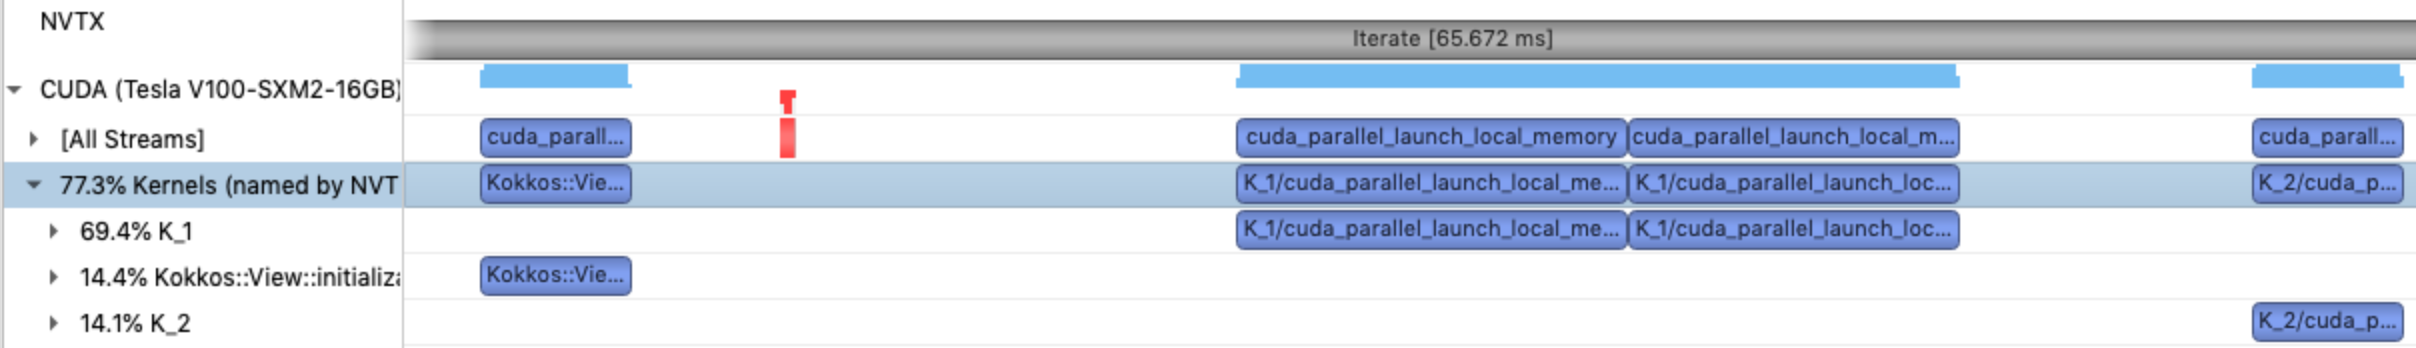
\includegraphics[width=\textwidth]{../figures/tools-simple-example-nvprof-zoomin.png}
\end{frame}



%==========================================================================

\begin{frame}[fragile]{Connecting to Tools - Vtune}
  To enable kernel renaming you need to:
  \begin{itemize}
    \item Load the vtune-connector via setting \texttt{KOKKOS\_TOOLS\_LIBS} in the run configuration.
    \item Choose the \texttt{Frame Domain / Frame / Function / Call Stack} grouping in the bottom up panel.
  \end{itemize}

  This does a few things:
  \begin{itemize}
    \item User Labels are now used as the primary name.
    \item You can expand to see individual kernel invocations
    \item You can dive further into an individual kernel invocation to see function calls within.
    \item Focus in on a kernel or individual invocation and do more detailed analysis. 
  \end{itemize}

  Also available: vtune-focused-connector:
  \begin{itemize}
    \item Used in conjunction with kernel-filter tool.
    \item Restricts profiling to a subset of kernels.
  \end{itemize}
\end{frame}

%==========================================================================

\begin{frame}[fragile]{Connecting to Tools - Vtune}
  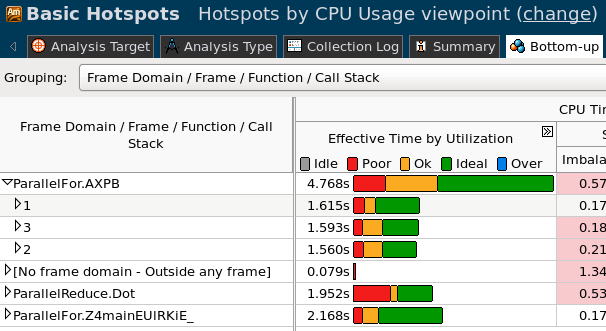
\includegraphics[width=\textwidth]{../figures/tools-vtune-example}

\end{frame}

%==========================================================================

\begin{frame}[fragile]{Connecting to Tools - Tau}
\textbf{TAU is a widely used Profiling Tool supporting most platforms.}

\vspace{5pt}
Tau supports:
\begin{itemize}
  \item profiling
  \item sampling
  \item tracing
\end{itemize}

\textbf{You do not need a connector tool for Tau!}

\vspace{5pt}
To enable TAU's Kokkos integration simply
\begin{itemize}
  \item \href{https://www.cs.uoregon.edu/research/tau/downloads.php}{Download} and install TAU
  \item Launch your program with \texttt{tau\_exec} (which will set \texttt{KOKKOS\_TOOLS\_LIBS} for you)
\end{itemize}

For questions contact tau-users@cs.uoregon.edu

\end{frame}

%==========================================================================

\begin{frame}[fragile]{Connecting to Tools - Tau}

Tau will use Kokkos instrumentation to display names and regions as defined by Kokkos:

	\vspace{10pt}
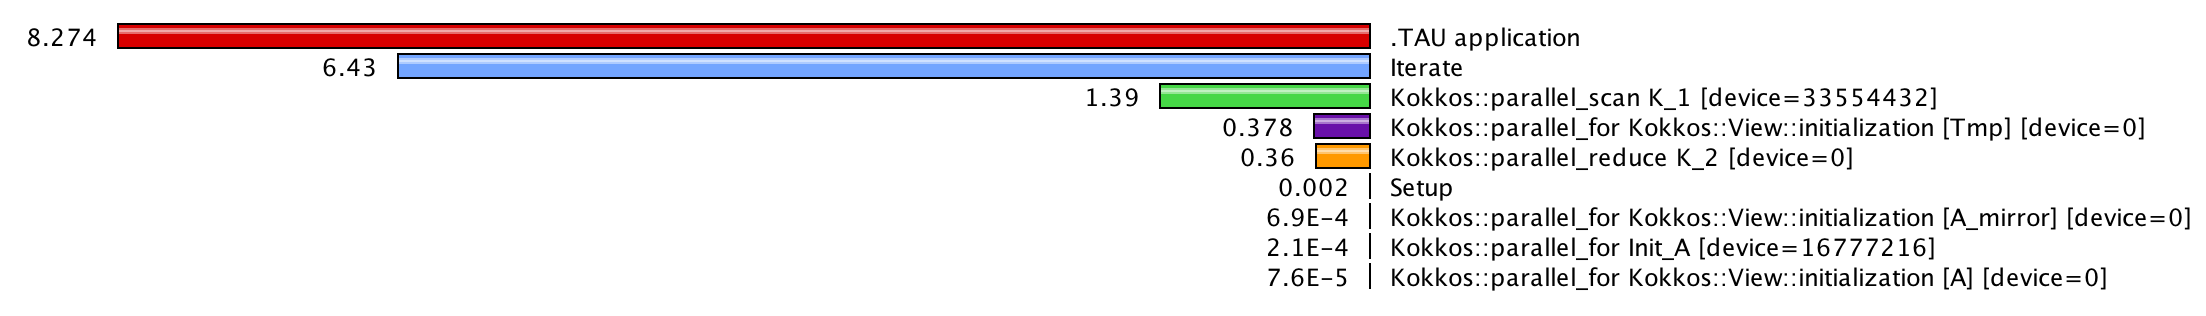
\includegraphics[width=\textwidth]{../figures/tools-simple-example-tau.png}
\end{frame}

\begin{frame}[fragile]{More Info on TAU}

\begin{center}
	In-depth tutorial: \url{http://www.nic.uoregon.edu/~khuck/kokkos/2024-Kokkos-Tuning-Tutorial/2024-Kokkos-Tools-Tutorial-TAU.pdf} 
\end{center}
	\begin{center} 
        Repo: \url{https://github.com/UO-OACISS/tau2} \\
	Contact: \url{tau-users@cs.uoregon.edu}
	\end{center} 
\end{frame}
%==========================================================================
\begin{frame}[fragile]{Timemory}
  \href{https://github.com/NERSC/timemory}{Timemory} is a modular toolkit provided by NERSC that aims to
  simplify the creation of performance analysis tools by providing a common design pattern
  of classes which encapsulate how to perform a start+stop/sample/entry of "something". 
  Each of these components (from timers to HW counters to other profilers) can be used 
  individually with zero overhead from the library. 
  It also provides wrappers and utilities for handling multiple components generically, data storage, 
  writing JSON, comparing outputs, etc. 

  \vspace{1em}
  As a by-product this design, the library
  provides an large set of individual profiling libraries whose usage comes with
  the same ease as using the simple-timer tool: setting \texttt{KOKKOS\_TOOLS\_LIBS}. 
%  \href{https://github.com/NERSC/timemory}{Timemory} is another multi architecture profiling tool.
%	
%Timemory provides:
%\begin{itemize}
%  \item a wide set of measurement capabilities.
%  \item avoid complicated environment variables.
%  \item different connector libraries for different tasks.
%  \item unique capabilities such as simultaneous CPU/GPU roofline modeling.
%\end{itemize}
%
%As with other Kokkos tools to use it:
%\begin{itemize}
%  \item	build the tools
%  \item set \texttt{KOKKOS\_TOOLS\_LIBS}
%\end{itemize}
%
\end{frame}


\begin{frame}[fragile]{Timemory}
  \begin{itemize}
  \item It also provides novel capabilities other tools don't, like simultaneous CPU/GPU
    roofline modeling. 
  \item The usage here is simple:
  \begin{itemize}
  \item \lstinline|spack install timemory +kokkos_tools +kokkos_build_config| \\
     \lstinline|[+mpi +cuda +cupti +papi +caliper ...]|
  \item Wait 3 months while spack builds every software package ever from scratch
  \item In \lstinline|<PREFIX>/lib/timemory/kokkos_tools/| there will be 5 to 30+ 
  Kokkos profiling libraries
  \end{itemize}
  \item Roofline modeling requires one additional setup
  \begin{itemize}
  \item \lstinline|timemory-roofline -T "TITLE" -t gpu_roofline -- <CMD>|
  \item Where everything after \lstinline|--| is just running your application
  \end{itemize}
  \item For more information: \url{https://github.com/NERSC/timemory}
  \end{itemize}
\end{frame}

\begin{frame}[fragile]{Timemory}
  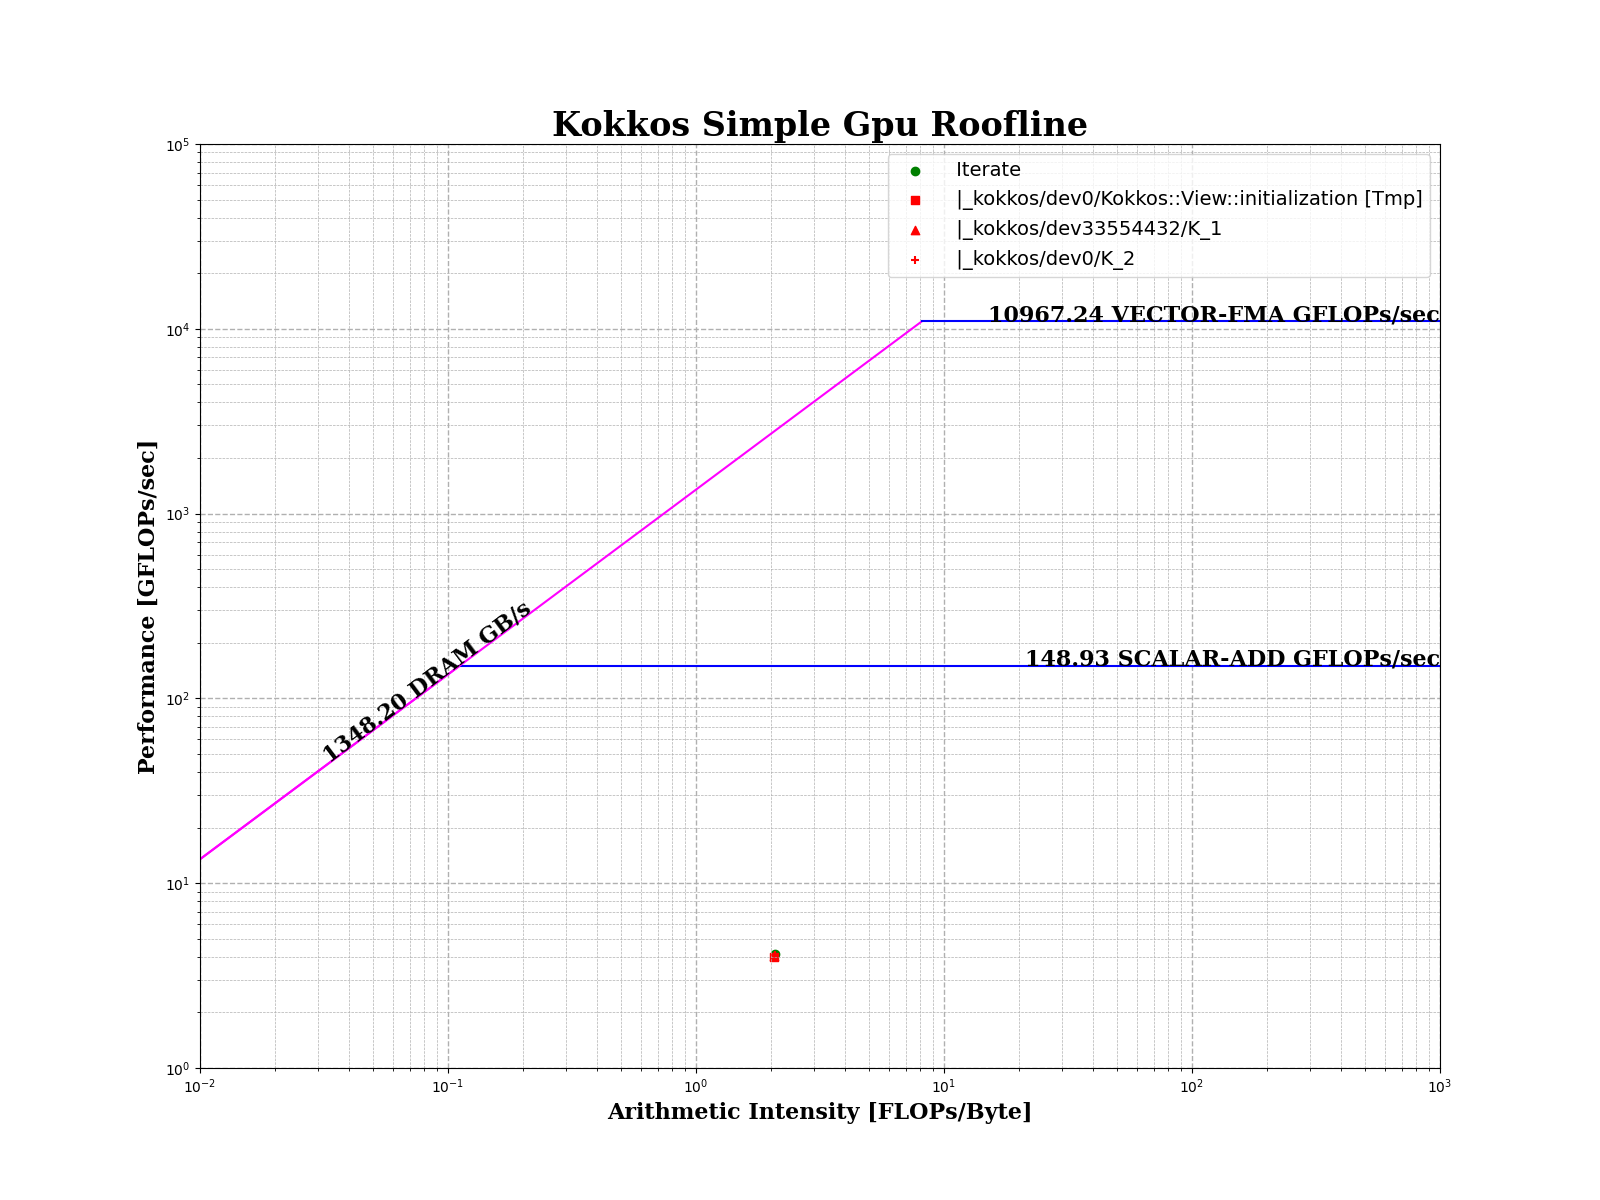
\includegraphics[width=\textwidth]{../figures/tools-simple-example-timemory.png}
\end{frame}

%==========================================================================

\begin{frame}[fragile]{Other}
  \begin{itemize}
    \item Caliper - Broad program analysis capabilities. UVM Profiling.
    \item HPCToolkit - Not a connector, but a sampling tool with great Kokkos support
  \end{itemize}

\end{frame}

%==========================================================================

\begin{frame}[fragile]{Connector Summary}
  \begin{itemize}
    \item Connectors inject Kokkos specific information into vendor and academic tools.
    \item Helps readability of profiles.
    \item Removes your need to put vendor specific instrumentation in your code.
    \item Growing list of tools support Kokkos natively.
  \end{itemize}
\end{frame}


%\begin{frame}{Kokkos Tools Quick Start}
\textbf{Learning Objectives:} 

\begin{itemize}
\item Quickly start using a tool via Kokkos Tools build system for any Kokkos application and backend.
\item Set environment variables of Kokkos Tools to customize its tools' behaviors.
\end{itemize}
\end{frame}


\begin{frame}{All the info so far is great...}
\begin{center}
I want to start using Kokkos Tools this minute for my use case. 
% <Optional text:>
% What's the tl;dr? 
\end{center}
\end{frame}

\begin{frame}[fragile]{Quick Start: Generic}
\begin{enumerate}
\small 
\item \textbf{Assume} an install prefix of your Kokkos build in \texttt{\$\{YOUR\_KOKKOS\}}.
\item \textbf{Obtain} via \texttt{git clone github.com/kokkos/kokkos-tools; cd kokkos-tools;} and load needed external software dependences.
\item \textbf{Install} with CMake:
\begin{lstlisting}
mkdir build; cd build; cmake ..
-DKokkos_ROOT="${YOUR_KOKKOS}"
-DCMAKE_INSTALL_PREFIX="${YOUR_KTO_INSTALL}";
make -j 4; make install;
\end{lstlisting}

\item \textbf{Set up} environment variables:
\begin{lstlisting}
export KOKKOS_TOOLS_GLOBAL<toolvar>=...
\end{lstlisting}
\item \textbf{Load} tool library via
\begin{lstlisting}
export KOKKOS_TOOLS_LIBS=
"${YOUR_KTO_INSTALL}/lib64/libkp_toolName.so"
\end{lstlisting}

\item \textbf{Run}: \texttt{cd /path/to/your/app; ./yourKokkosApp.exe};
\end{enumerate}

\end{frame}

\begin{frame}[fragile]{Quick Start: \texttt{nvtx-connector} on Perlmutter}

\begin{enumerate}
\small 

\item \textbf{Assume} an install prefix of Kokkos with the CUDA backend enabled in \texttt{\${YOUR\_KOKKOS}}.\\
\item \textbf{Obtain}
\begin{lstlisting}
git clone https://github.com/kokkos/kokkos-tools;
cd kokkos-tools; module load PrgEnv-gnu;
\end{lstlisting}
\item \textbf{Install} with CMake:
\begin{lstlisting}
mkdir build; cd build; cmake ..
-DKokkos_ROOT="${YOUR_KOKKOS}"
-DCMAKE_INSTALL_PREFIX="/where/to/install/the/tools";
make -j 4; make install;
\end{lstlisting}

\item \textbf{Set up}: 
\begin{lstlisting} 
export KOKKOS\_TOOLS\_GLOBALFENCES=1;
\end{lstlisting}

\item \textbf{Load}:
\begin{lstlisting}
export KOKKOS_TOOLS_LIBS=
"/where/to/install/the/tools/lib64/libkp_nvtx_connector.so";
\end{lstlisting}

\item \textbf{Run}: \texttt{cd /path/to/your/app; ncu -o profile ./yourKokkosApp.exe;}
\end{enumerate}
\end{frame}


\begin{frame}[fragile]{Additional Notes}
	\begin{enumerate}
	   \item For the latest default version of Kokkos Tools, make sure you are on the develop branch of the github repository and do a git pull.
	   \item Use \texttt{ccmake ..} instead of \texttt{cmake ..} for Kokkos Tools to see the list of Kokkos Tools options available.
	\end{enumerate}
\end{frame}


\begin{frame}[fragile]{Summary of Quick Start Guide}
To quickly start using a tool in Kokkos Tools for your Kokkos application, you do the following via git and CMake:
\begin{enumerate}
\item \textbf{Assume} an appropriate build of Kokkos is available.
\item \textbf{Obtain} the latest version of Kokkos Tools.
\item \textbf{Install} Kokkos Tools on your machine.
\item \textbf{Set up} installed tool libraries through specifying values for environment variables.
\item \textbf{Load} the Kokkos Tools tool library or libraries you want to use.
\item \textbf{Run} your Kokkos application, as usual.
\end{enumerate}

\begin{center}
\small See \url{https://github.com/kokkos/kokkos-tools/blob/develop/README.md}
for the latest. 
\end{center}

\end{frame}



\begin{frame}[fragile]

  {\Huge Tuning}

  \vspace{10pt}

  {\large Using Kokkos' autotuning hooks.}

  \vspace{20pt}

  \textbf{Learning objectives:}
  \begin{itemize}
    \item {Why do we need tuning?}
    \item {What are Input and Output Variables?}
    \item {How to register parameters for tuning.}
    \item {Using the APEX Tuner.}
    \item {Using the Apollo Tuner.}
  \end{itemize}

  \vspace{-20pt}

\end{frame}

%==========================================================================


\begin{frame}[fragile]{Why Tuning?}
Lets look at the canonical implementation for SPMV in Kokkos:
\begin{code}[keywords={int,parallel_for,auto,parallel_reduce,TeamThreadRange,TeamPolicy,ThreadVectorRange,double}]
int rows_per_team = ...;
parallel_for("SPMV",TeamPolicy<>(nrows/rows_per_team,
  team_size,vector_length),
  KOKKOS_LAMBDA(auto const team_t& team) {
  int start_row = team.league_rank()*rows_per_team;
  parallel_for(
    TeamThreadRange(team,start_row,start_row+rows_per_team),
    [&](int row) {
      int idx_begin = a.offsets(row); 
      int idx_end = a.offsets(row+1);
      parallel_reduce(ThreadVectorRange(team,idx_begin,idx_end),
      [&](int i, double& lsum) {
        lsum += A.value(i) * x(A.idx(i));
      },y(row));
    }); 
  });
\end{code}
\end{frame}

\begin{frame}[fragile]{Why Tuning?}
There are three free parameters which determine performance:
 
\hspace{10pt} \textbf{rows\_per\_team} \hspace{10pt} \textbf{team\_size} \hspace{10pt} \textbf{vector\_length}

\vspace{5pt}
These parameters depend most on three factors:
\begin{itemize}
  \item Which architecture are you on?
  \item How many rows are in A?
  \item How many non-zeros are in A?
\end{itemize}
\end{frame}

%==========================================================================

\begin{frame}[fragile]{Why Tuning}
\textbf{Finding the right parameters is a daunting task.}

Heuristics are possible, but they have to change all the time
\begin{itemize}
  \item KokkosKernels' heuristic for NVIDIA K80 failed on V100
  \item Now AMD GPUs and Intel GPUs are coming. 
\end{itemize}

\pause
\vspace{10pt}
What if you could auto tune these parameters instead?

\vspace{5pt}
What information would you need to provide and what comes out? Need:

\pause
\vspace{5pt}
\begin{itemize}
  \item Context information, such as problem sizes.
  \item To be able to provide multiple inputs of different types.
  \item To tune multiple correlated parameters.
  \item Different tuning strategies in different areas.
\end{itemize}

\pause
\begin{block}{Kokkos Tuning}
Kokkos Tuning provides a flexible runtime auto tuning interface.
\end{block}
\end{frame}


\begin{frame}[fragile]{Tuning a Parameter}
\textbf{Kokkos' Tuning Infrastructure is very flexible.}

\pause
\vspace{5pt}
\textit{Which makes it right now more complex than is desirable.}

We will glance over some aspects here and give you the most important info for simple tuning tasks.

\pause
\vspace{10pt}
Kokkos Tuning has four fundamental concepts:
\begin{itemize}
  \item \texttt{Input-Types}: Descriptors for the type of input information for tuning tasks
  \item \texttt{Output-Types}: Descriptors of output variables for tuning tasks
  \item \texttt{Variable-Values}: Instances of \texttt{Input-Types} or \texttt{Output-Types}
  \item \texttt{Contexts:} Marker for tuning scopes. 
\end{itemize}
\end{frame}

\begin{frame}[fragile]{Types}
The types for input variables and output variables describe what makes sense to do with a variable
\begin{itemize}
  \item Not types in the C++ sense
  \item These types can contain runtime information such as candidate sets.
\end{itemize}

\pause
\vspace{5pt}
\textbf{Huh? Where is this coming from?}

Think about the different optimization spaces of variables:
\begin{itemize}
\item Discrete sets, only specific values make sense: e.g. vector length 2, 4, 8, 16
\item Continuous ranges, all values in a range $0-N$ are valid.
\item Statistical semantics, is the search space logarithmic or linear?
\end{itemize}

Often you'll have a simple case, for which we will provide helper functions.

\pause
\textbf{Tuning Variables (both input and output) need to accomodate these situations.}

\vspace{5pt}
\textit{We will discuss this later}
\end{frame}

\begin{frame}[fragile]{Tuning a single variable}
\textit{Kokkos Provided API will be highlighted, and is in the namespace \texttt{Kokkos::Tools::Experimental}}

\vspace{5pt}
\textbf{Start by creating the types (helper functions discussed later):}
\begin{code}
std::vector<int64_t> candidates = {0, 3, 7, 11};
size_t tuning_candidate_type_id = 
  create_tuning_output_type("values",candidates);
size_t tuning_input_type_id = 
  create_tuning_input_type("kernels");
\end{code}

\textbf{Next create variables for the inputs:}
\begin{code}[keywords={VariableValue,make_variable_value}]
VariableValue input_A = 
  make_variable_value(tuning_input_type_id,"A");
VariableValue input_B = 
  make_variable_value(tuning_input_type_id,"B");
\end{code}

\textbf{The actual tuning region is scoped through a context:}
\begin{code}[keywords={get_new_context_id,begin_context,end_context}]
size_t context_1 = get_new_context_id();
begin_context(context_1);
// This is the tuned region
end_context(context_1);
\end{code}
\end{frame}


\begin{frame}[fragile]{Tuning a single variable}
The context scope defines both the timing for the tuning operation and the scope in which to set input variables and obtain output (tuned) variables:

\begin{code}[keywords={get_new_context_id,begin_context,end_context,set_inpute_values,request_output_values,set_input_values}]
size_t context_1 = get_new_context_id();
begin_context(context_1);
set_input_values(context_1, 1, &input_value_A);
request_output_values(context_1, 1, &tuned_value);
end_context(context_1);
\end{code}

\pause
In this case we used a \texttt{Categorical} input value
\begin{itemize}
  \item Essentially just marks a code path as used here.
  \item But for SPMV optimal vector length depends on row lengths!
  \begin{itemize}
    \item If there is only 1 matrix: categorical works
    \item Else need numerical input value, where output mapping depends on input potentially not just as a lookup.
  \end{itemize}
\end{itemize}

\pause
We also only used one input and one output value:
\begin{itemize}
	\item Interface takes pointers to arrays for multiple \texttt{VariableValue}!
\end{itemize}
\end{frame}

%==========================================================================

\begin{frame}[fragile]{Helper Functions}

The code we demonstrated before used helper functions. We'll show their
implementation to help demonstrate some details.

\begin{code}[keywords={get_new_context_id,begin_context,end_context,VariableInfo,
	               StatisticalCategory,kokkos_value_catgorical,ValueTYpe,
		       kokkos_value_int64,kokkos_value_double,valueQuantity,CandidateValueType,
		       kokkos_value_set,make_candidate_set,declare_output_type}]
template <class T>
size_t create_tuning_output_type(
    const char* name,
    std::vector<T>& candidate_values) {
  using Kokkos::Tools::Experimental;
  VariableInfo tuningVariableInfo;
  tuningVariableInfo.category =
      StatisticalCategory::kokkos_value_categorical;
  tuningVariableInfo.type = std::is_integral<T>::value ?
      ValueType::kokkos_value_int64 :
      ValueType::kokkos_value_double;
  tuningVariableInfo.valueQuantity =
      CandidateValueType::kokkos_value_set;
  tuningVariableInfo.candidates = make_candidate_set(
      candidate_values.size(),
      candidate_values.data());  
  return declare_output_type(name, tuningVariableInfo);
}
\end{code}
\end{frame}
\begin{frame}[fragile]{Helper Functions Continued}

\begin{code}[keywords={get_new_context_id,begin_context,end_context,VariableInfo,
	               StatiscalCategory,kokkos_value_categorical,kokkos_value_string,
		       kokkos_value_unbounded,declare_inpute_type,valueQuantity}]
size_t create_tuning_input_type(const char* name) {
  using Kokkos::Tools::Experimental;
  VariableInfo info;
  info.category = StatisticalCategory::kokkos_value_categorical;
  info.type = ValueType::kokkos_value_string;
  info.valueQuantity = kokkos_value_unbounded;
  return declare_input_type(name, info);
}
\end{code}


\end{frame}

\begin{frame}[fragile]{APEX: Runtime Auto-tuning for Kokkos Applications} 
\begin{itemize}
   \item APEX: Autonomic Performance Environment for eXascale 
   \item Associated with TAU profiling library, reusing its codebase.
   \item Provides auto-tuning during Kokkos application's execution, e.g., at every invocation of a \texttt{Kokkos::parallel\_for()}
   \item Search for best-performing tuning parameter values via simulated annealing or genetic search. 
\end{itemize}

\pause
How to use APEX:\\
	\begin{code}[mathescape=false]
apex_exec --apex:kokkos-tuning ./Executable.exe ARGS
\end{code}
\end{frame}

\begin{frame}[fragile]{APEX Speeds Up Kokkos Applications}

\begin{figure}
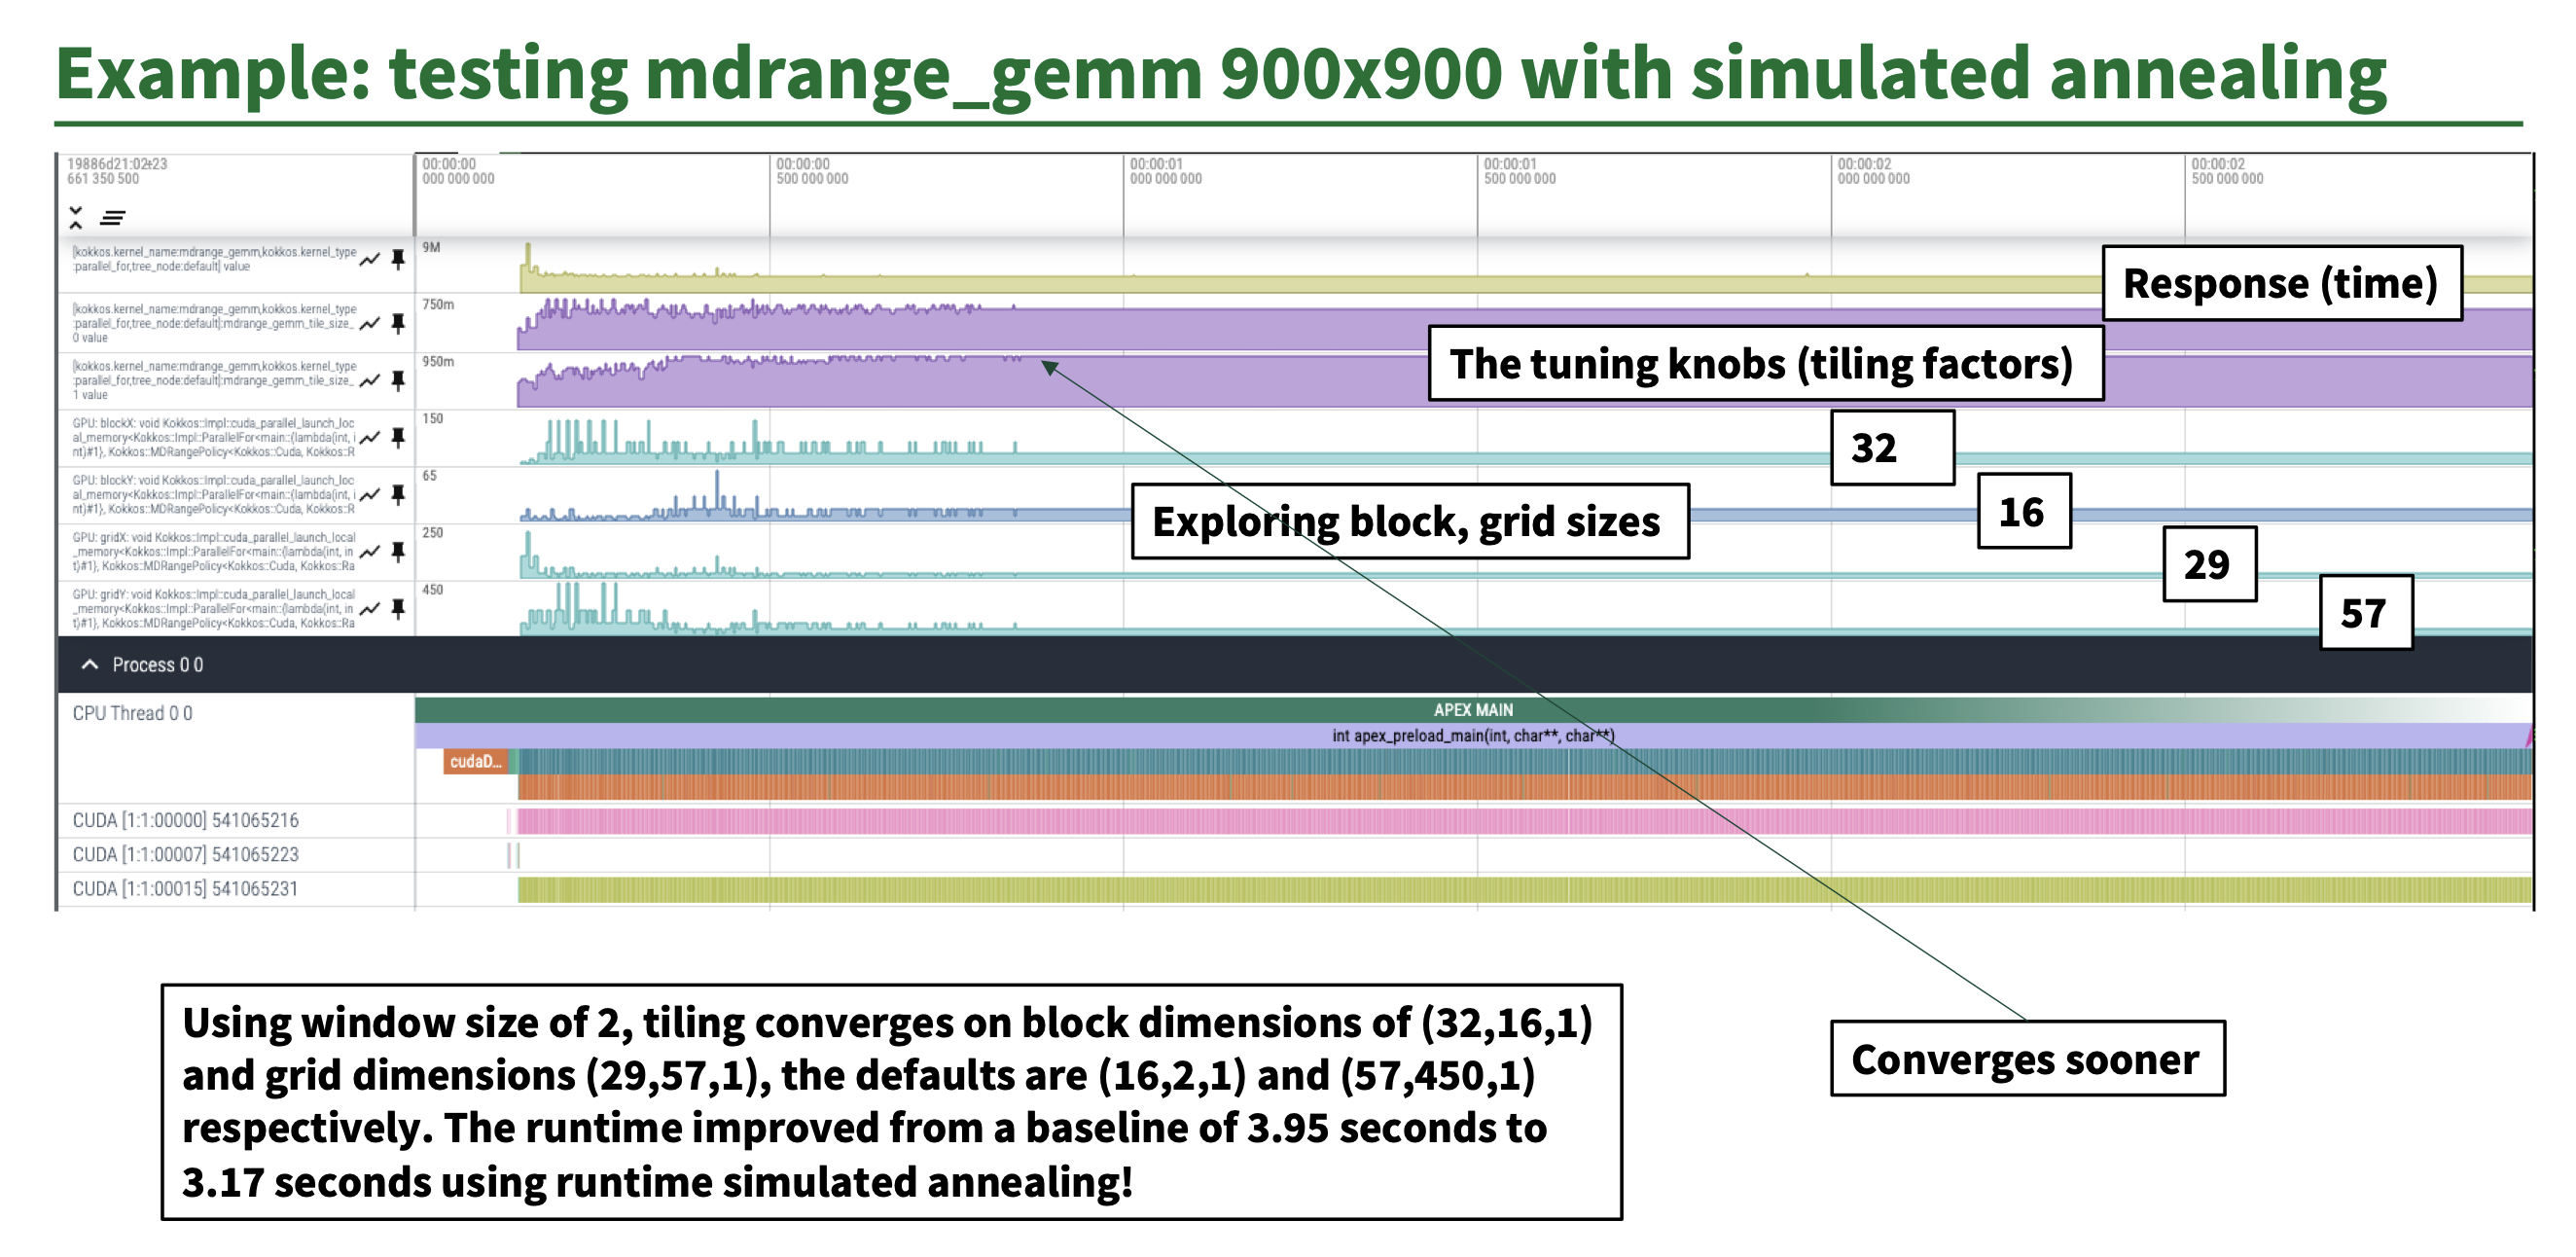
\includegraphics[width=\textwidth]{../figures/apextuningplot.png}
\end{figure}

\end{frame} 

\begin{frame}[fragile]{APEX In-depth}

\begin{center}
In-depth tutorial: \\
	\small \url{http://www.nic.uoregon.edu/~khuck/kokkos/2024-Kokkos-Tuning-Tutorial/2024-Kokkos-Tools-Tutorial-APEX.pdf}
\end{center}

\begin{center}
	Repo: \url{https://github.com/UA-OACISS/apex} \\	
	Email: \url{khuck@cs.uoregon.edu}
\end{center}

\end{frame}

\begin{frame}[fragile]{Apollo: a Prototype Tuning Tool}
  \textbf{Apollo: A model driven auto tuning tool}

\begin{itemize}
  \item Feature-rich tuning tool targeting this interface.
  \item Builds decision tree based models to find best-performing parameter values.
  \item Can retrain models if observed and expected performance deviate.
  \item Can save models for subsequent runs.
\end{itemize}

\pause
How to use Apollo:
	\begin{code}[mathescape=false]
export KOKKOS_TOOLS_LIBS=${APOLLO_PATH}/libapollo-tuner.so
./Executable.exe ARGS
\end{code}
\end{frame}

%======================================================================

\begin{frame}[fragile]{Some Results from the KokkosKernels Test Suite}
  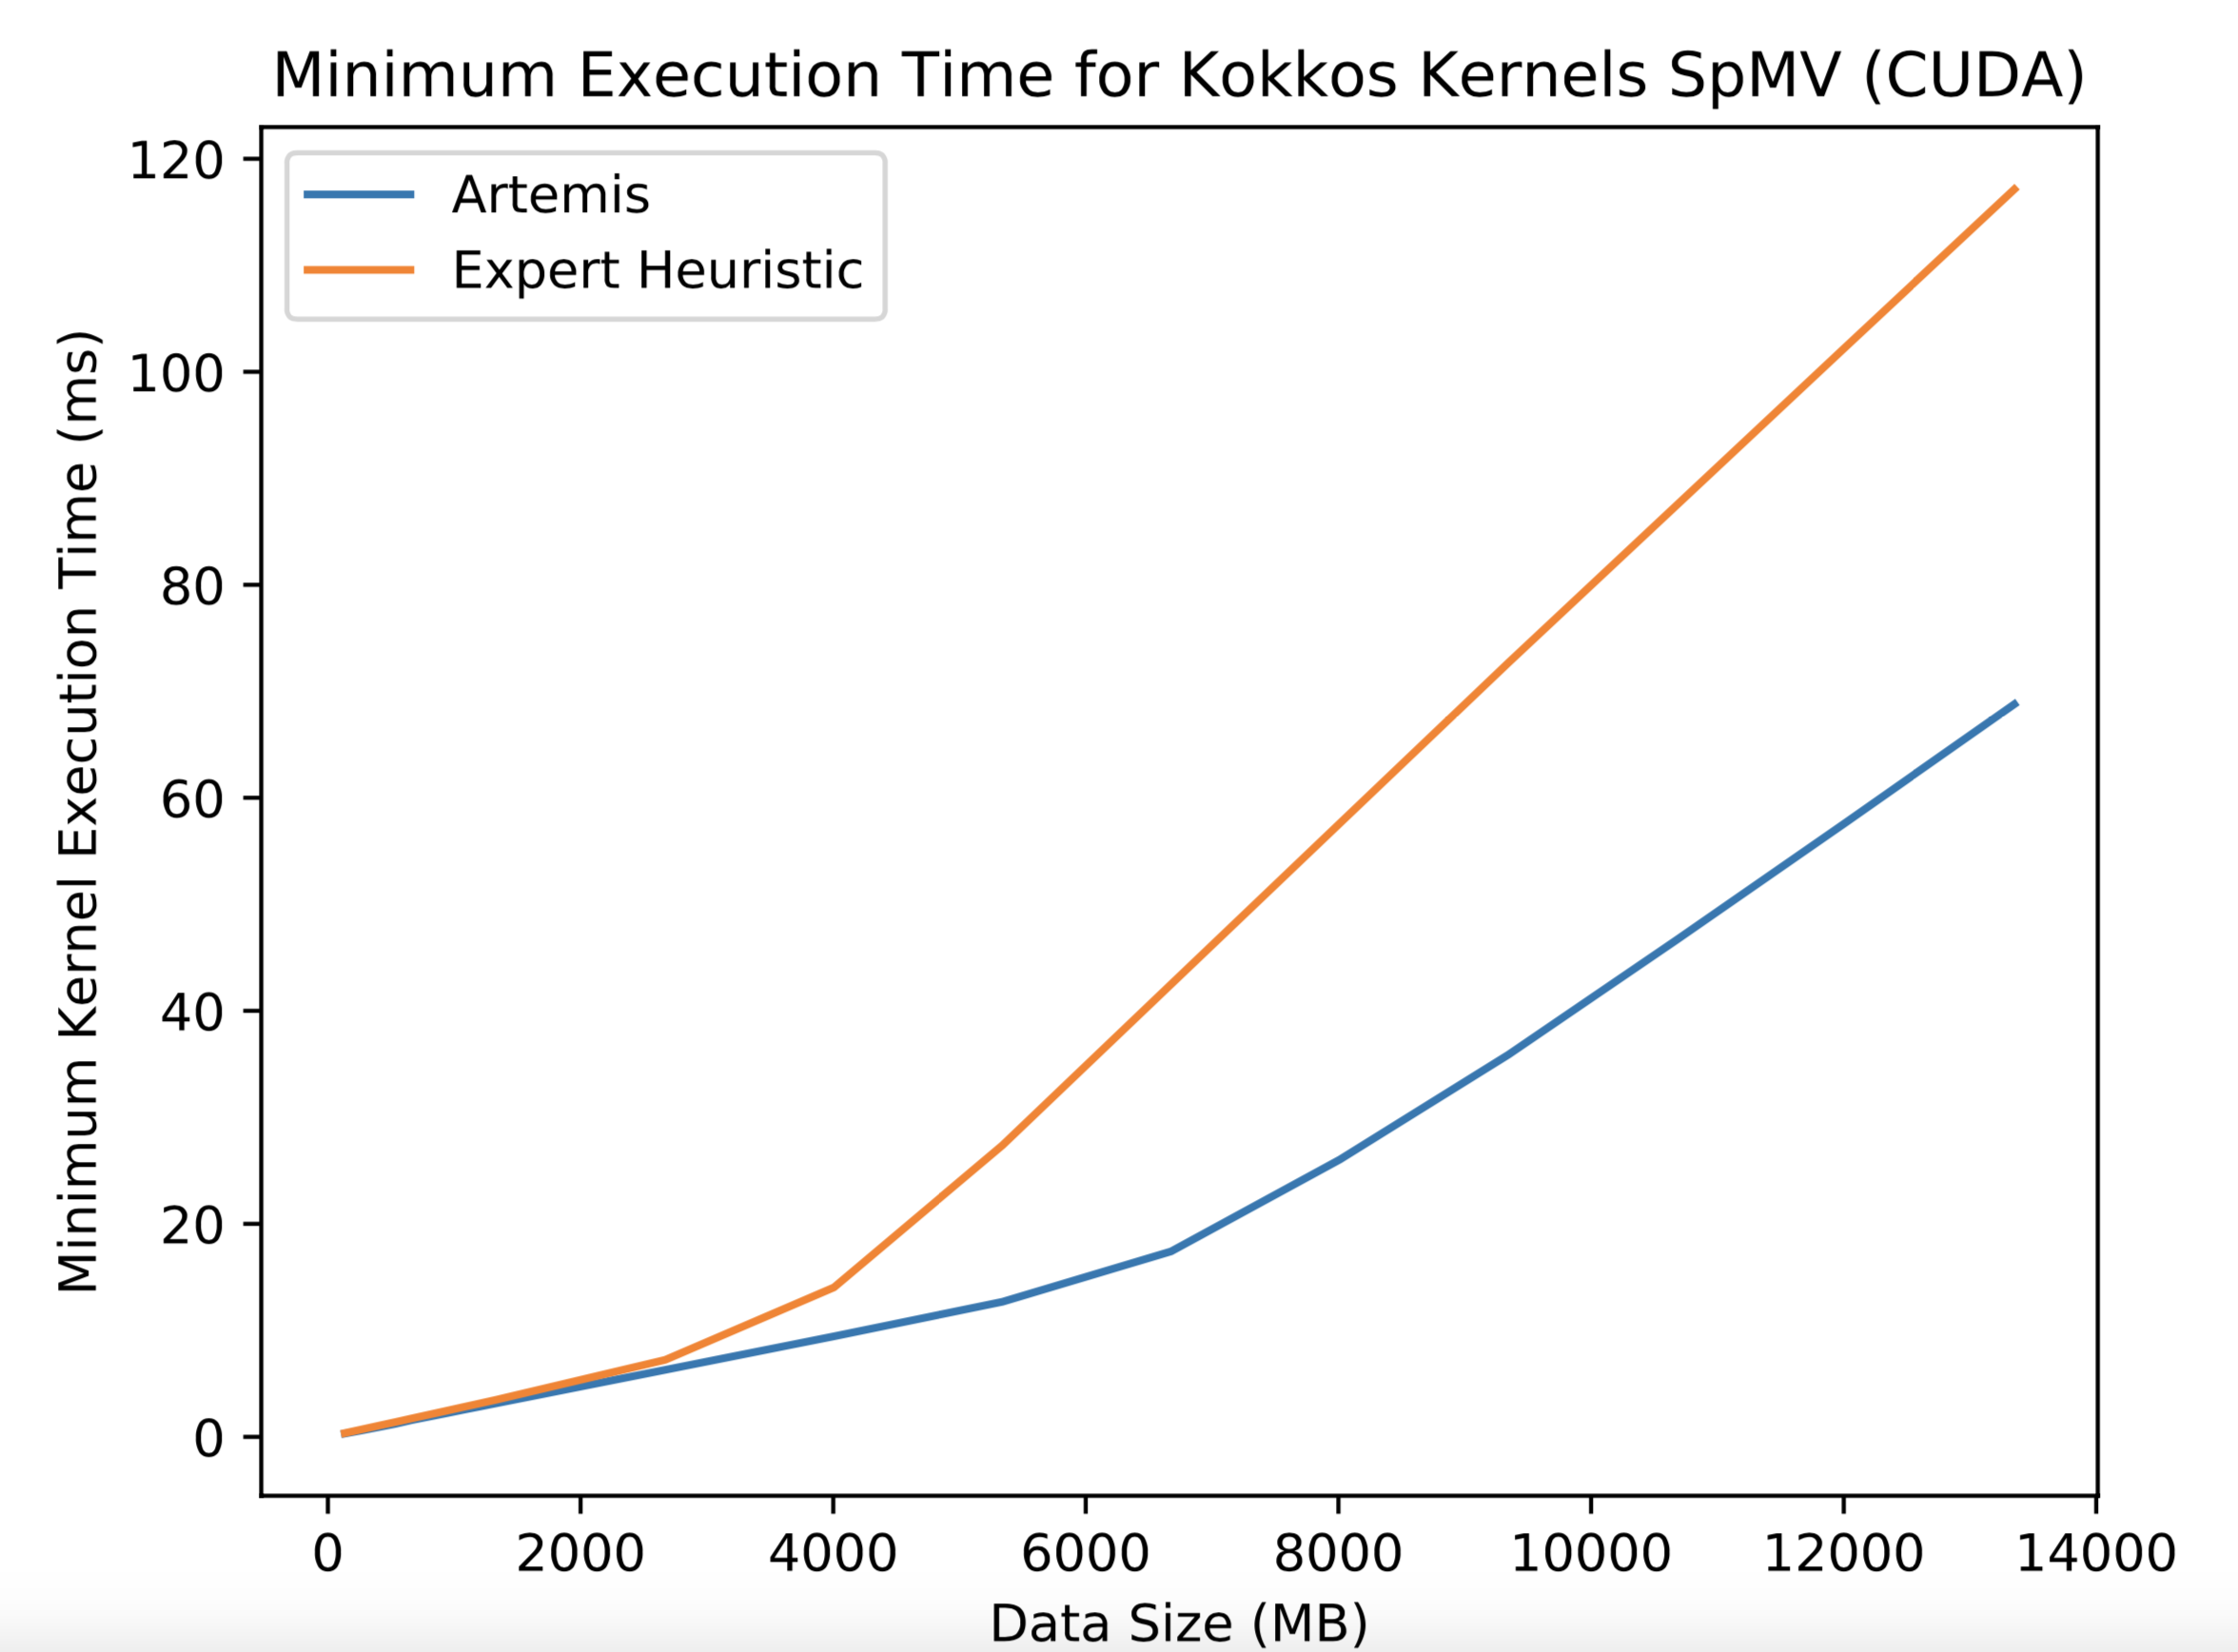
\includegraphics[width=0.9\textwidth]{../figures/apollo.png}
\end{frame}

\begin{frame}[fragile]{More Information on Apollo}

\begin{center} 
\textbf{Apollo Project Page:} \url{https://computing.llnl.gov/projects/apollo} \\
\end{center} 

\begin{center}
\textbf{Repo}: \url{https://github.com/LLNL/apollo} \\
\textbf{Contact}: \url{georgakoudis1@llnl.gov}
\end{center} 

\end{frame}

%==========================================================================

\begin{frame}[fragile]{Rules for Tuning}
  \begin{itemize}
    \item Load the output value array you pass to request\_output\_values
	    with sane defaults. If the tool doesn't overwrite them, your
	    program shouldn't crash. This protects you from a tool-free
	    situation
    \item No choice from your set/range of candidates should crash your
	    program. Options can be slow, but must all be functional
    \item Call set\_input\_values and request\_output\_values only once per context. 
  \end{itemize}
\end{frame}

\begin{frame}[fragile]{Future: Built-in Tuning}
For the future we plan on allowing automatic internal tuning of things like:
\begin{itemize}
  \item Team Size and Vector Length for \texttt{TeamPolicy}
  \item Tile Sizes for \texttt{MDRangePolicy}
  \item CUDA block size of \texttt{RangePolicy}
  \item Occupancy of kernels.
\end{itemize}
\begin{code}
parallel_for("A",TeamPolicy<>(N,AUTO,AUTO), ... );
parallel_for("B",MDRangePolicy<>({0,0},{N0,N1},{AUTO,AUTO}), ... );
\end{code}

\pause
But often more context is needed:
\begin{itemize}
  \item Kokkos on its own has limited information: Label, Iteration Range, and Kernel Type ID.
  \item SPMV: can't distinguish two matrices with same row count but vastly different row lengths.
  \item Stencil: can't distinguish runtime stencil depth.
\end{itemize}
\end{frame}


%==========================================================================

\begin{frame}[fragile]{Tuning Summary}
\textbf{Kokkos Tuning Hooks enable more performance portability}
\begin{itemize}
  \item Avoid figuring out the right heuristic for every platform.
  \item Will be more valuable when targeting Intel, NVIDIA and AMD GPUs as well as ARM, Intel, IBM and AMD CPUs!
\end{itemize}

\textbf{The app provides input variables to describe the context}
\begin{itemize}
  \item Input variables are descriptors of the problem scope.
  \item Categorical, Ranges, Sets are possible.
  \item Describe scaling for Ranges such as logarithmic or linear for categorizing problems.
\end{itemize}

\textbf{The app requests output variables}
\begin{itemize}
  \item Same type system as input variables.
  \item Enables the description of the search space for tools.
\end{itemize}

\end{frame}


\begin{frame}[fragile]

  {\Huge Custom Tools}

  \vspace{10pt}

  {\large How to write your own tools for the KokkosP interface.}

  \vspace{20pt}

  \textbf{Learning objectives:}
  \begin{itemize}
    \item {The KokkosP hooks}
    \item {Callback registration inside the application}
    \item {Throwaway debugging tools}
  \end{itemize}

  \vspace{-20pt}

\end{frame}

%==========================================================================

\begin{frame}[fragile]{Motivation}

KokkosTools also allow you to write your own tools!

\begin{itemize}
  \item Implement a simple C interface.
  \item Only implement what you want to use!
  \item Full access to the entire instrumentation.
\end{itemize}

\vspace{10pt}
But why would I want to do that?

\begin{itemize}
  \item Profiling tools which know about your code structure and properly categorize information.
  \item Add in situ analysis hooked into your CI system.
  \item Write debugging tools specific for your framework.
  \item Write throwaway debugging tools for larger apps, instead of recompiling.
\end{itemize}

\pause
\textit{We will first walk through the hooks and then illustate with an example.}
\end{frame}

%==========================================================================

\begin{frame}[fragile]{Infrastructure and Initialization}
\textbf{Some Helper Classes}
\begin{code}
// Contains a unique device identifier.
struct KokkosPDeviceInfo { uint32_t deviceID; };

// Unique name of execution and memory spaces.
struct SpaceHandle { char name[64]; };
\end{code}

\pause
\textbf{Initialization and Finalization hooks}
\begin{code}[keywords={extern,void,int,uint64_t,uint32_t}]
extern "C" void kokkosp_init_library(
  int loadseq, uint64_t version, uint32_t num_devinfos,
  KokkosPDeviceInfo* devinfos);
\end{code}
\vspace{-15pt}
  \begin{itemize}
    \item Called during \texttt{Kokkos::initialize}
    \item Provides device ids used subsequently.
    \item Use this call to setup tool infrastructure.
  \end{itemize}
\begin{code}[keywords={extern,void,int,uint64_t,uint32_t}]
extern "C" void kokkosp_finalize_library();
\end{code}
\vspace{-15pt}
  \begin{itemize}
    \item Called during \texttt{Kokkos::finalize}
    \item Usually used to output results.
  \end{itemize}
\end{frame}

%==========================================================================

\begin{frame}[fragile]{Parallelism Hooks}
\begin{code}[keywords={extern,void,int,uint64_t,uint32_t,const,char}]
extern "C" {
  void kokkosp_begin_parallel_for(const char* name,
                                  uint32_t devid,
                                  uint64_t* kernid);
  void kokkosp_begin_parallel_reduce(const char* name,
                                     uint32_t devid,
                                     uint64_t* kernid);
  void kokkosp_begin_parallel_scan(const char* name,
                                   uint32_t devid,
                                   uint64_t* kernid);
};
\end{code}
\vspace{-15pt}
\begin{itemize}
  \item Called when a parallel dispatch is initiated.
  \item \texttt{name} is the user provided string or a typeid.
  \item \texttt{kernid} is set by the tool to match up with the \texttt{end} call.
\end{itemize}

\begin{code}[keywords={extern,void,int,uint64_t,uint32_t,const,char}]
extern "C" void kokkosp_end_parallel_for(uint64_t kernid);
extern "C" void kokkosp_end_parallel_reduce(uint64_t kernid);
extern "C" void kokkosp_end_parallel_scan(uint64_t kernid);
\end{code}
\vspace{-15pt}
\begin{itemize}
  \item Called when a parallel dispatch is done.
  \item \texttt{kernid} is the value the begin call set.
\end{itemize}
\end{frame}

%==========================================================================

\begin{frame}[fragile]{Memory Hooks}
\begin{code}[keywords={extern,void,int,uint64_t,uint32_t,const,char}]
extern "C" void kokkosp_begin_deep_copy(
  SpaceHandle dst_hndl, const char* dst_name, const void* dst_ptr,
  SpaceHandle src_hndl, const char* src_name, const void* src_ptr,
  uint64_t size);
\end{code}
\begin{itemize}
  \item Called when a \texttt{deep\_copy} is started.
  \item Provides space handles, names, ptrs and size of allocations.
\end{itemize}

\begin{code}[keywords={extern,void,int,uint64_t,uint32_t,const,char}]
extern "C" void kokkosp_end_deep_copy();
\end{code}
\begin{itemize}
  \item Called when a \texttt{deep\_copy} is done.
\end{itemize}

\begin{code}[keywords={extern,void,int,uint64_t,uint32_t,const,char}]
extern "C" void kokkosp_allocate_data(SpaceHandle hndl,
  const char* name, void* ptr, uint64_t size);
extern "C" void kokkosp_deallocate_data(SpaceHandle hndl,
  const char* name, void* ptr, uint64_t size);
\end{code}
\begin{itemize}
  \item Called when allocating or deallocating data.
\end{itemize}
\end{frame}

%==========================================================================

\begin{frame}[fragile]{Callback Registration}
Sometimes it is useful to build a tool into an executable.

\vspace{5pt}
\begin{block}{Callback Registration}
Kokkos Tools provide a callback setting system to set tool callbacks from within the application.
\end{block}

Takes the form of:
\begin{code}
void set_HOOK_callback(HOOK_FUNCTION_PTR callback);
\end{code}

Where \texttt{HOOK} is one of 
\begin{code}
init finalize push_region pop_region begin_parallel_for 
end_parallel_for begin_parallel_reduce end_parallel_reduce
begin_parallel_scan end_parallel_scan begin_fence end_fence
allocate_data deallocate_data begin_deep_copy end_deep_copy
\end{code}

One can also store a callback set, reload it and pause tool calls
\begin{code}
EventSet get_callbacks();  void set_callbacks(EventSet);
void pause_tools();        void resume_tools();
\end{code}
\end{frame}

\begin{frame}[fragile]{Callback Registration}
Example:
\begin{lstlisting}[language=C++]
#include <Kokkos_Core.hpp>
using Kokkos::Profiling;
using Kokkos::Tools::Experimental;
using Kokkos;

void kokkosp_allocate_data(SpaceHandle space,
  const char* label, const void* const ptr, uint64_t size) {
  printf("Allocate: [%s] %lu\n",label,size);
}
void kokkosp_deallocate_data(SpaceHandle space,
  const char* label, const void* const ptr, uint64_t size) {
  printf("Deallocate: [%s] %lu\n",label,size);
}

int main(int argc, char* argv[]) {
  initialize(argc, argv);
  set_allocate_data_callback(kokkosp_allocate_data);
  set_deallocate_data_callback(kokkosp_deallocate_data);
  ...
  finalize();
}
\end{lstlisting}

\end{frame}

%==========================================================================

\begin{frame}[fragile]{Example: Throwaway Debugging Tool}
Sometimes you just need to know what is in a View before and after entering a kernel for the 5th time:
\begin{itemize}
  \item The view is on the GPU and its on some rank of a large run.
  \item Recompiling the app takes hours.
\end{itemize}

\pause
\vspace{10pt}
\textbf{Simple Kokkos tool could do it!}

What we need:
\begin{itemize}
  \item Store the pointer and size of the view with a specific label when it gets allocated.
  \item Print the View when entering a kernel and before exiting it. 
  \item Make sure the view didn't get deallocated in the mean time. 
\end{itemize}
\end{frame}

\begin{frame}[fragile]{Example: Throwaway Debugging Tool}
Store the pointer:
\vspace{-2pt}
\begin{code}[keywords={int,uint64_t,extern,void,const,char,void,if}]
int* data; uint64_t N; int count;
extern "C" void kokkosp_allocate_data(SpaceHandle handle,
  const char* name, void* ptr, uint64_t size) {
  if(strcmp(name,"PuppyWeights")==0) {
    data = (int*)ptr+32; N = size; count = 0;
}}
\end{code}

Print the View:
\vspace{-2pt}
\begin{code}[keywords={int,uint64_t,extern,void,const,char,void,if,else}]
void print_data() { 
  std::vector<int> hcpy(N);
  cudaMemcpy(hcpy.data(),data,N*sizeof(int));
  for(int i=0;i<N;++i) printf("(%d %d)",i,hcpy[i]); printf("\n");
}
extern "C" void kokkosp_begin_parallel_for(const char* name, 
  uint32_t, uint64_t* kernid) {
  if(strcmp(name,"PuppyOnCouch")==0) { 
    count++; if(count==5) print_data(); *kernid=1;
  } else { *kernid = 0; } 
}
extern "C" void kokkosp_end_parallel_for(uint64_t kernid) {
  if(kernid == 1 && count==5) print_data();
}
\end{code}

\end{frame}

\begin{frame}[fragile]{TestCode}
\begin{code}[keywords={int,uint64_t,extern,void,const,char,void,parallel_for,for,initialize,finalize}]
#include <Kokkos_Core.hpp>
#include <cmath>

int main(int argc, char* argv[]) {
  Kokkos::initialize(argc, argv);
  {
    int N = argc > 1 ? atoi(argv[1]) : 12;
    int R = argc > 2 ? atoi(argv[2]) : 10;
    Kokkos::View<double*> a("PuppyWeights",N);

    for(int r=0; r<R; r++) {
      Kokkos::parallel_for("PuppyOnCouch",N,KOKKOS_LAMBDA(int i)
                           { a(i) = i*r; });
    }
  }
  Kokkos::finalize();
}
\end{code}

Output:
\begin{code}
(0 0) (1 4) (2 8) (3 12)
(0 0) (1 5) (2 10) (3 15)
\end{code}
\end{frame}

\begin{frame}[fragile]{Hooks Summary}
\textbf{Implementing your own tools is easy!}
\begin{itemize}
  \item Simply implement the needed C callback functions.
  \item Only implement what you need.
  \item Goal is to make it simple enough so that one-off tools are a viable debugging help.
\end{itemize}

\vspace{10pt}
\textbf{Callback registration for applications}
\begin{itemize}
  \item The callback registration system allows to embed tools in applications.
  \item Store callback sets and restore them.
\end{itemize}

\end{frame}


%==========================================================================

\begin{frame}[fragile]
  
  \vspace{-10pt}
  {\Huge Clang Based Static Analysis}
  \vspace{20pt}

  \textbf{\ul{Goals of this section}}
  \begin{itemize}
    \item {Introduce The Possibility Of Kokkos Specific Warnings}
    \item {Show The Three Classes Of Errors We Can Detect}
    \item {Show You How To Use Them}
    \item {List Current/Planned Warnings}
  \end{itemize}
\end{frame}

%==========================================================================

\begin{frame}[fragile]{Kokkos Specific Warnings}
  
  \textbf{\ul{Can We Have Kokkos Specific Warnings}}
  even if the current configuration compiles?
  \begin{code}[linebackgroundcolor={\btLstHL{6}{darkred!20}},
      keywords={}, frame=single
    ]
void fooOOPS(int i) { printf("%i\n", i); }

int main(int argc, char **argv) {
  // Initialize  ...
  Kokkos::parallel_for(15, KOKKOS_LAMBDA(int i) {
       fooOOPS(i);
      });
  }
  // Finalize ...
}
  \end{code}

\pause
\textbf{Answer: Yes, now we can.}
\end{frame}

%==========================================================================

\begin{frame}[fragile]
  
  \begin{code}[linebackgroundcolor={\btLstHL{6}{darkred!20}},
      keywords={}, frame=single
    ]
void fooOOPS(int i) { printf("%i\n", i); }

int main(int argc, char **argv) {
  // Initialize  ...
  Kokkos::parallel_for(15, KOKKOS_LAMBDA(int i) {
       fooOOPS(i);
      });
  }
  // Finalize ...
}
  \end{code}

  \textbf{Using clang-tidy}

  \begin{code}[linebackgroundcolor={
      },
      keywords={}, frame=single
    ]
> clang-tidy -checks=-*,kokkos-* file.cpp
    <file:line:col> @redwarning@red: Function 'fooOOPS' called in 
                         a lambda was missing 
                         KOKKOS_X_FUNCTION annotation.
         fooOOPS(i);
         ^
<file:line:col> note: Function 'fooOOPS' was delcared here
void fooOOPS(int i) { printf("%i\n", i); }
  \end{code}

\end{frame}

%==========================================================================

\begin{frame}[fragile]{Types Of Errors}
  
\textbf{Could become compiler errors}
\begin{code}[linebackgroundcolor={}, keywords={}, frame=single]
void fooOOPS(int i) { printf("%i\n", i);}
KOKKOS_FUNCTION void foo(){fooOOPS(1);}
\end{code}

\textbf{Could become runtime crashes}
\begin{code}[linebackgroundcolor={ }, keywords={}, frame=single]
struct bar {
  int baz;
  void foo(){parallel_for(15, KOKKOS_LAMBDA(int){baz;});}
};
\end{code}

  \textbf{\color{red}Will produce incorrect results}
\begin{code}[linebackgroundcolor={ }, keywords={}, frame=single]
double foo(){
  double d;
  auto func = KOKKOS_LAMBDA(int i, @reddouble sum@red){sum += i;};
  parallel_reduce(15, func, d);
  return d;
}
\end{code}

\end{frame}

%==========================================================================

\begin{frame}[fragile]{Getting Started}
  
  \textbf{\ul{How to use}}
  \begin{itemize}
    \item \textbf{Code:} \href{https://github.com/kokkos/llvm-project}{kokkos/llvm-project}
    \item \textbf{Build:} \href{https://llvm.org/docs/CMake.html}{llvm build instructions}
    \item \textbf{Run:} The same way you would normally use clang-tidy, except with kokkos checks enabled. 
  \end{itemize}
  
\end{frame}

%==========================================================================

\begin{frame}[fragile]{Using Kokkos Checks}
  
  \textbf{\ul{Usage Examples: With Cmake}}
  \begin{code}[linebackgroundcolor={\btLstHL{6-7}{darkred!20}},
      keywords={}, frame=single]
#! /bin/bash

cmake \
  /path/to/kokkos/code/you/want/to/build \
  -DKokkos_ROOT="/path/to/installed/kokkos" \
  -DCMAKE_EXPORT_COMPILE_COMMANDS=ON \
  -DCMAKE_CXX_CLANG_TIDY="clang-tidy;-checks=kokkos-*"
  \end{code}

  The above will:
  \begin{itemize}
    \item make a compile\_commands.json file that clang-tidy and clangd can use
    \item invoke clang-tidy on all of the files compiled by the CXX compiler
  \end{itemize}
  If the kokkos clang-tidy is not in the path you will need to put the full
  path to it.
  
\end{frame}

%==========================================================================
\begin{frame}[fragile]{Using Kokkos Checks}
  
  \textbf{\ul{Usage Examples: Invoke clang-tidy directly}}
  \begin{code}[linebackgroundcolor={
      },
      keywords={}, frame=single
    ]
> clang-tidy -checks=-*,kokkos-* file.cpp
    <file:line:col> @redwarning@red: Function 'fooOOPS' called in 
                         a lambda was missing 
                         KOKKOS_X_FUNCTION annotation.
         fooOOPS(i);
         ^
<file:line:col> note: Function 'fooOOPS' was delcared here
void fooOOPS(int i) { printf("%i\n", i); }
  \end{code}

  Assumes that we have the compile\_commands.json file from the previous slide either in the current directory or in a parent directory. 
\end{frame}

%==========================================================================
\begin{frame}[fragile]{Using Kokkos Checks}
  
  \textbf{\ul{Usage Examples: As part of clangd}}
  \begin{code}[linebackgroundcolor={},
      keywords={}, frame=single
    ]
void fooOOPS(int i) { printf("%i\n", i); }

int main(int argc, char **argv) {
  // Initialize  ...
  Kokkos::parallel_for(15, KOKKOS_LAMBDA(int i) {
       fooOOPS(i); @orangeFunction 'fooOOPS' called in lambda...@orange
      });
  }
  // Finalize ...
}
  \end{code}

  \href{https://clangd.llvm.org/}{clangd is a language server that can work with many editors via a plugin.}

  \vspace{20pt}

  \href{https://github.com/kokkos/kokkos-tutorials/blob/main/LectureSeries/KokkosTutorial_07_ClangSA.mp4}{Video Demo Of Clang Tools}

\end{frame}

%========================================================================== 
\begin{frame}[fragile]{Existing and Planned Checks}
  
  {\huge State of The Tool}

  \textbf{\ul{Current Checks}}
  \begin{itemize}
    \item Ensure KOKKOS\_FUNCTION (the one you saw here)
    \item KOKKOS\_LAMBDA captures implicit this
  \end{itemize}

  \textbf{\ul{Beta and planned checks}}
  \begin{itemize}
    \item parallel\_reduce functor takes argument by reference
    \item Nested reference lambda capture const behavior
    \item Unallowed types like std::vector in Kokkos contexts
    \item Force users to provide names for kernels
  \end{itemize}

  \textbf{\ul{Your Issue?}}
  \begin{itemize}
      \item \textbf{Send us your requests:} \href{https://github.com/kokkos/llvm-project}{kokkos/llvm-project}
  \end{itemize}
\end{frame}


\begin{frame}[fragile]{Module 7: Summary}

\textbf{Kokkos Tools:}
\begin{itemize}
  \item Kokkos Tools provide an instrumentation interface \textbf{KokkosP} and \textbf{Tools} to leverage it.
  \item The interface is \textbf{always available} - even in release builds.
  \item Zero overhead if no tool is loaded during the run.
  \item Dynamically load a tool via setting \texttt{KOKKOS\_TOOLS\_LIBS} environment variable.
  \item Set callbacks in code for tools compiled into the executable. 
\end{itemize}

\textbf{Kokkos Connector Tools:}
\begin{itemize}
  \item Connectors inject Kokkos specific information into vendor and academic tools.
  \item Helps readability of profiles.
  \item Removes need to put vendor specific instrumentation in codes.
  \item Growing list of tools support Kokkos natively.
\end{itemize}
\end{frame}

\begin{frame}[fragile]{Module 7: Summary}
\textbf{Kokkos Tuning Hooks enable more performance portability}
\begin{itemize}
  \item Avoid figuring out the right heuristic for every platform.
  \item Input variables descripte the problem scope.
  \item Output variables descripe the search space.
\end{itemize}

\textbf{Implementing your own tools is easy!}
\begin{itemize}
  \item Simply implement the needed C callback functions.
  \item Only implement what you need.
  \item The callback registration system allows to embed tools in applications.
\end{itemize}

\textbf{Static Analysis}
\begin{itemize}
  \item Have semantic checks going beyond C++ errors.
  \item Integrates into your editors.
\end{itemize}
\end{frame}

\begin{frame}{Module 8: Outlook (09/04)}
	\textbf{KokkosKernels Dense Linear Algebra}

	\textbf{KokkosKernels Sparse Linear Algebra}

	\textbf{KokkosKernels Sparse Solvers}

	\textbf{KokkosKernels Graph Kernels}


	\vspace{5pt}
	\textbf{Don't Forget:} Join our Slack Channel and drop into our office hours on Tuesday.
	
	\vspace{5pt}
	\textbf{Updates at:} \href{https://kokkos.link/the-lectures-updates}{kokkos.link/the-lectures-updates}
	
	\vspace{5pt}
	\textbf{Recordings/Slides:} \href{https://kokkos.link/the-lectures}{kokkos.link/the-lectures}

\end{frame}
\end{document}

